\documentclass[11pt]{article}
\usepackage[a4paper,margin=2.4cm]{geometry}
\usepackage[T1]{fontenc}
\usepackage[utf8]{inputenc}
\usepackage{lmodern,microtype,amsmath,amssymb,bm,graphicx,booktabs,array,longtable,xcolor,hyperref}
\newcolumntype{L}[1]{>{\raggedright\arraybackslash}p{#1}}
\emergencystretch=2em
\hypersetup{colorlinks=true,linkcolor=blue!45!black,citecolor=blue!45!black,urlcolor=blue!45!black,
pdfauthor={Thomas D. Kuehne; Alexander Cerjan; Vladislav Efremkin; Hermann Schulz-Baldes; Emil Prodan}}
\newcommand{\CPtwoK}{\textsc{CP2K}}
\newcommand{\Quickstep}{\textsc{Quickstep}}
\newcommand{\ii}{\mathrm{i}}
\newcommand{\dd}{\mathrm{d}}
\newcommand{\bk}{\bm{k}}
\newcommand{\br}{\bm{r}}
\newcommand{\bR}{\bm{R}}
\newcommand{\bG}{\bm{G}}
\newcommand{\bb}{\bm{b}}
\newcommand{\Tr}{\operatorname{Tr}}
\newcommand{\Pf}{\operatorname{Pf}}
\newcommand{\Sig}{\operatorname{Sig}}
\newcommand{\BZ}{\mathrm{BZ}}
\numberwithin{equation}{section}
\title{Topological Systems with CP2K}
\author{Thomas D. K\"uhne$^{a,b,c,*}$, Alexander Cerjan$^{d}$,\\
Vladislav Efremkin$^{a,b}$, Hermann Schulz-Baldes$^{e}$, and Emil Prodan$^{f}$\\[0.6em]
\small $^{a}$Center for Advanced Systems Understanding (CASUS),\\
\small Untermarkt 20, D-02826 G\"orlitz, Germany\\
\small $^{b}$Helmholtz-Zentrum Dresden-Rossendorf (HZDR),\\
\small Bautzner Landstrasse 400, D-01328 Dresden, Germany\\
\small $^{c}$Chair of Computational Systems Science, Institute of Artificial Intelligence,\\
\small Technische Universit\"at Dresden, D-01069 Dresden, Germany\\
\small $^{d}$Center for Integrated Nanotechnologies, Sandia National Laboratories,\\
\small Albuquerque, New Mexico 87185, USA\\
\small $^{e}$Department Mathematik, Friedrich-Alexander-Universit\"at Erlangen-N\"urnberg,\\
\small Cauerstrasse 11, D-91058 Erlangen, Germany\\
\small $^{f}$Department of Physics, Yeshiva University, New York, USA\\[0.4em]
\small $^{*}$Corresponding author: \href{mailto:tkuehne@cp2k.org}{tkuehne@cp2k.org}}
\date{}
% Target journal: Computer Physics Communications.
% Affiliations, contribution statements and final submission scope require author approval.
\begin{document}
\maketitle
\begin{abstract}
Electronic transport and topology probe information that cannot be
inferred from band energies alone. Current operators, inter-state
overlaps, symmetry representations, and the spatial structure of a
Hamiltonian must be treated consistently. We formulate these quantities
in the nonorthogonal Gaussian atomic-orbital representation of \CPtwoK,
connecting finite-temperature Kubo transport, Wilson-loop and Chern
analysis, crystalline symmetry representations, spectral localizers, and
the quadratic pseudospectrum. The overlap metric is retained in operator
products, symmetry transformations, and spectral-gap estimates.
Real-space and reciprocal-space constructions share Hamiltonian,
position, and spin--orbit matrix elements without requiring a fitted
Wannier Hamiltonian. Dense reference calculations are complemented by
distributed sparse assembly, symmetric-indefinite inertia calculations,
and an optional sparse Pfaffian backend. We explain how the finite
matrix formulations relate to noncommutative geometry and distinguish
local topological protection from an electronic band gap or a mobility
gap. Wilson and inversion calculations, native projective little-group
and antiunitary corepresentation tests, and serial/MPI operator
comparisons provide complementary validation.
The implementation scope is stated explicitly: the current Kubo path
evaluates symmetric dissipative DC response. Crystalline analysis
includes nonsymmorphic endpoint-to-line compatibility, but a complete
space-group EBR classifier and universal symmetry reduction of
topological properties remain development targets.
\end{abstract}
\noindent\textbf{Keywords:} CP2K, Kubo transport, noncommutative geometry,
spectral localizer, topological quantum chemistry, spin--orbit coupling
\par\medskip
\noindent\textit{Working manuscript for Computer Physics Communications.
Implementation and validation status: 24 September 2026.}
\clearpage
\section{Introduction}
Electronic-structure theory supplies a Hamiltonian and a Hilbert-space
representation; extracting transport or topological information requires
additional structure. Two calculations can agree in their eigenvalues
while disagreeing in matrix elements of position, current, or a symmetry
operator. This distinction is especially important in a localized
nonorthogonal basis, where ordinary matrix multiplication is not the
representation of operator composition.

The \Quickstep{} module of \CPtwoK{} combines localized Gaussian orbitals
with plane-wave and multigrid representations of densities and
electrostatics \cite{Kuehne2020CP2K,Lippert1997,Lippert1999,VandeVondele2005a}.
This representation provides access to spatially resolved operators
without first fitting a tight-binding Hamiltonian. It also creates
specific obligations: the AO metric, periodic image indices, Bloch
convention, nonlocal pseudopotentials, and spinor ordering must remain
consistent across every analysis.

The first-principles transport programme of K\"uhne, Heske and Prodan
\cite{KuehneTransport2020} supplies an important starting point:
thermally disordered structures are treated as configurations of a
covariant family of Hamiltonians, and dissipation is included in the
finite-temperature response. Bellissard's operator-algebraic framework
connects this viewpoint to topology without assuming exact translation
symmetry of each configuration \cite{Bellissard1994,ProdanSchulzBaldes2016}.
The present manuscript combines this motivation with reciprocal-space
invariants and spatially resolved finite-matrix diagnostics.

The scope is deliberately broader than a band-topology interface.
Wilson loops resolve the geometry of an isolated band subspace;
crystalline representations resolve symmetry constraints; a localizer
tests an energy-position query; a quadratic pseudospectrum produces
approximately localized states; and Kubo response determines a
transport coefficient at specified temperature and dissipation.
None of these outputs can simply be substituted for another.

The companion study on symmetry-reduced k-point sampling and Wannier
analysis develops the underlying Bloch reconstruction and full-mesh
export. We repeat the operator conventions needed to make the present
article self-contained, but keep the detailed topology, transport, and
localizer analysis here. In particular, Wannier90 is an optional route
to a reduced representation, not a prerequisite for native AO analysis.
Sections below distinguish implemented algorithms from the more general
theory and from extensions still requiring validation.
The materials-discovery applications discussed later are distinguished
from our small test and demonstration calculations: the former motivate
the scientific use of these methods, while the latter establish specific
numerical identities and illustrate their operation.
\section{Hamiltonians and operators in a nonorthogonal basis}
\label{sec:operators}
\subsection{Covariant matrices and the physical metric}
Let $\Phi$ denote the row of basis functions $|\phi_\mu\rangle$, and
$|\psi\rangle=\Phi c$. Define
\begin{equation}
 S=\Phi^\dagger\Phi,\qquad
 H=\Phi^\dagger\widehat H\Phi,\qquad
 X_a=\Phi^\dagger\widehat r_a\Phi .
 \label{eq:ao-data}
\end{equation}
The overlap must be positive definite on the retained basis, and the
normalization is $c^\dagger Sc=1$. The generalized eigenproblem is
\begin{equation}
 HC=SC\varepsilon,\qquad C^\dagger SC=I .
 \label{eq:generalized}
\end{equation}
A covariant matrix $A$ acts on coefficient vectors through $S^{-1}A$.
Consequently, composition of two \emph{projected} operators is represented
by $AS^{-1}B$, and the projected commutator by
$AS^{-1}B-BS^{-1}A$. An ordinary product $AB$ is generally incorrect.

For a nonsingular change of basis $\Phi'=\Phi T$,
\begin{equation}
 S'=T^\dagger ST,\quad A'=T^\dagger AT,\quad c'=T^{-1}c .
 \label{eq:basis-change}
\end{equation}
The expectation $c^\dagger Ac$ and the generalized spectrum are unchanged.
The orthonormal representation
$\widetilde A=S^{-1/2}AS^{-1/2}$ is useful for proofs and dense reference
calculations. It need not be formed in a sparse implementation: products
can be evaluated by solving linear systems with $S$.

A finite-basis projection is not an algebra homomorphism for arbitrary
continuum operators. With $\Pi=\Phi S^{-1}\Phi^\dagger$,
$\Phi^\dagger\widehat A\Pi\widehat B\Phi$ differs in general from
$\Phi^\dagger\widehat A\widehat B\Phi$.
Thus a commutator or a variance of projected positions is an observable
of the projected model, not automatically its complete-basis continuum
counterpart. This distinction is monitored through basis convergence
rather than hidden in a numerical tolerance.

\subsection{Finite positions and AO export}
For an isolated system, analytic Gaussian first moments provide
$X_a$ in the same basis ordering as $H$ and $S$. Translation of the
coordinate origin by $x_a$ gives $X_a-x_aS$, not $X_a-x_aI$.
Likewise an energy query uses $H-ES$. These two simple identities are
essential for origin and energy-shift invariance.

The \texttt{AO\_MATRICES} print section can export overlap, scalar KS
Hamiltonian, and the three position matrices. They permit an independent
finite-Hamiltonian calculation. Activating SOC in a property section
does not silently turn the separate scalar KS export into a spinor
Hamiltonian export. Model Hamiltonians can use the low-level matrix
kernels when the metric, positions, and symmetry structure are supplied
consistently; this does not imply automatic adapters for every
electronic-structure method.

\subsection{Bloch operators and directed overlaps}
In the cell Fourier convention,
\begin{equation}
 H_{\mu\nu}(\bk)=\sum_{\bR}e^{\ii\bk\cdot\bR}H_{\mu\nu}(\bR),
 \qquad
 S_{\mu\nu}(\bk)=\sum_{\bR}e^{\ii\bk\cdot\bR}S_{\mu\nu}(\bR).
 \label{eq:bloch-matrices}
\end{equation}
Here $\bk$ is Cartesian and includes inverse-length units; fractional
reciprocal coordinates instead require $2\pi$ in the phase.
Image-cell labels cannot be discarded before forming derivatives or
inter-k-point connections.

For cell-periodic states and a directed step $\bb$, the occupied-state
overlap is
\begin{equation}
 M(\bk,\bb)=C^\dagger(\bk)O(\bk+\bb;\bb)C(\bk+\bb),\qquad
 O_{\mu\nu}=\sum_{\bR}e^{\ii(\bk+\bb)\cdot\bR}
 \langle\phi_{\mu0}|e^{-\ii\bb\cdot\br}|\phi_{\nu\bR}\rangle .
 \label{eq:wannier90-mmn-definition}
\end{equation}
The zero-step limit is $S(\bk)$, but a finite link is not obtained by
replacing $O$ with $S$, or by simply contracting coefficient vectors.
Neighbor lists, reciprocal-boundary phases, and the selected band rank
are part of the observable. Wannier90's file and library interfaces can
consume such data \cite{Pizzi2020}; native Wilson calculations need no
Wannier localization or interpolation.

\subsection{Spin--orbit coupling and symmetry}
The implementations considered here start from a converged scalar
restricted SCF potential and add GTH spin--orbit matrix elements.
The localizer and Bloch-Kubo paths use the complete AO spinor space,
whereas a second-variational band-topology calculation uses a selected
scalar-state space whose size must be converged separately.
Neither construction is self-consistent noncollinear SOC DFT.

In spin-major ordering, the overlap is
$\mathbb S=\operatorname{diag}(S,S)$ and physical time reversal is
$\Theta=JK$, where
\begin{equation}
 J=\begin{pmatrix}0&I\\-I&0\end{pmatrix},\qquad
 \Theta^2=-I .
\end{equation}
Time-reversal relations must be checked for the Hamiltonian, metric,
and relevant operators; the presence of an SOC pseudopotential alone
does not establish them.
A Cartesian spatial rotation $R$ acts on spin through an SU(2) lift of
$\det(R)R$, with inversion acting trivially on spin and separately on
orbital parity. The sign ambiguity of this lift is retained in the
double-group multiplication law.

\section{Noncommutative geometry and physical interpretation}
\label{sec:ncg}
\subsection{Covariance rather than exact order}
For a family of configurations $\omega\in\Omega$, a spatial action
$\tau_a$ is represented by
\begin{equation}
 U_a H_\omega U_a^{-1}=H_{\tau_a\omega}.
 \label{eq:covariance}
\end{equation}
This covariance is weaker than $[U_a,H_\omega]=0$: a displaced thermal
configuration need not have the symmetries of its probability measure.
Bellissard's formulation replaces the Brillouin-zone description by
an algebra of such covariant observables with a trace per physical
volume \cite{Bellissard1994}. The operator-algebraic viewpoint therefore
remains meaningful when a single Bloch momentum is not a good quantum
number.

For sufficiently local observables, the trace per volume has the
schematic realization
\begin{equation}
 \mathcal T(A)=
 \lim_{V\rightarrow\infty}\frac{1}{V}
 \Tr(\chi_V A_\omega\chi_V),
 \label{eq:trace-volume}
\end{equation}
with the appropriate orbital trace and a physical-volume normalization.
Ergodicity supplies the conditions under which a typical large
configuration and an ensemble average agree. It does not guarantee
that a particular small simulation cell has self-averaged.

The first-principles construction must preserve covariance while
passing from continuum KS operators to AO matrices
\cite{KuehneTransport2020}. The metric is part of that transformation.
In a finite AO space, traces of projected covariant matrices use
$\Tr(S^{-1}A)$; traces of products use the intervening metric factors.
For local traces the spatial cutoff itself is an operator, not merely
an arbitrary subset of coefficient indices.

\subsection{Derivations, Fermi projections, and Chern pairings}
Choose spatial derivations
$\nabla_a A=-\ii[X_a,A]$ in an orthonormal representation.
For the Fermi projection $P=\mathbf1_{(-\infty,E_F)}(H)$, a
two-dimensional Chern pairing can be written, with a fixed orientation,
as
\begin{equation}
 C=2\pi\ii\,\mathcal T\!\left(P[\nabla_1P,\nabla_2P]\right)
   =-2\pi\ii\,\mathcal T\!\left(P[[X_1,P],[X_2,P]]\right).
 \label{eq:nc-chern}
\end{equation}
The trace normalization and oriented coordinates are chosen so that
the periodic limit agrees with the Berry-curvature convention used
below. Reversing that orientation reverses $C$.
Index theory relates such pairings to stable integers under the
required locality and gap or localization assumptions
\cite{ProdanSchulzBaldes2016}. Equation~\eqref{eq:nc-chern} is a theoretical
connection, not a claim that the current implementation evaluates a
general thermodynamic-limit noncommutative Chern formula.

The metric also enters a finite real-space evaluation. Let
$C_{\mathrm{occ}}$ contain occupied coefficients with
$C_{\mathrm{occ}}^\dagger S C_{\mathrm{occ}}=I$. The mixed-index
projector and position operators are
\begin{equation}
 \Pi=C_{\mathrm{occ}}C_{\mathrm{occ}}^\dagger S,\qquad
 \mathsf X_a=S^{-1}X_a,\qquad \Pi^2=\Pi.
 \label{eq:mixed-fermi-projector}
\end{equation}
Here $X_a$ denotes the covariant AO matrix of the position operator.
For a physical bulk window $w(\mathbf r)$, define its covariant
matrix $W_{\mu\nu}=\langle\phi_\mu|w|\phi_\nu\rangle$,
$\mathsf W=S^{-1}W$, and the area
$A_w=\int w(\mathbf r)\,\mathrm d^2r$. A finite-window version of
Eq.~\eqref{eq:nc-chern} is
\begin{equation}
 C_w=-\frac{2\pi\ii}{A_w}\,
 \Tr\!\left(\mathsf W\Pi
   [[\mathsf X_1,\Pi],[\mathsf X_2,\Pi]]\right).
 \label{eq:finite-window-chern}
\end{equation}
All mixed-index matrices transform by similarity under a nonsingular
AO basis change. This preserves the trace without assigning a local
contribution to an arbitrary subset of basis coefficients.
The area is a spatial measure, not a count of occupied states or AOs.
In an open finite model with commuting position matrices the trace
over the entire sample cancels between bulk and boundary contributions.
A bulk window instead permits comparison with the local Chern marker
\cite{BiancoResta2011}. A finite value need not be exactly quantized.
Projected AO positions need not commute, so the lattice cancellation
identity must not be imposed on an incomplete continuum basis.

The complex finite-window evaluator uses metric solves and checks
occupied-state orthonormality and $0\leq W\leq S$. Its finite-system
Quickstep interface integrates two-dimensional Gaussian windows
analytically over the AOs, with widths $\sigma_1,\sigma_2$ and area
$A_w=2\pi\sigma_1\sigma_2$. The projector is defined by an explicit
energy in a resolved gap, not by smeared SCF occupations.
Open-boundary model and GPW/GAPW controls are provided in the
Supporting Information. This spatial diagnostic complements rather
than duplicates Wilson-loop or $\mathbb Z_2$ analysis.

Periodic boundaries require a separate treatment. Finite-torus
approximations periodize the spatial derivations rather than applying
an unbounded Cartesian position to a periodic cell
\cite{Prodan2013,BauMarrazzo2024}. Such approximate derivations do not
generally obey an exact Leibniz rule at finite size. Differentiating
the finite Fermi matrix and replacing that derivative by a spectral
Fermi divided difference times a Hamiltonian derivative are therefore
distinct finite-size procedures. Hall and Chern crosschecks must
retain this distinction, the order of tensor indices, and the relative
orientation of the Berry and Clifford constructions.

A spectral gap excludes eigenvalues in an interval. A mobility gap
instead concerns localization and transport even when states are
present. A localizer gap is the smallest singular value of a composite
energy-position operator. These three gaps answer different questions.
The localizer is useful precisely because spatially resolved
information can remain available where a bulk band classification is
not directly applicable \cite{Dixon2023}. Its numerical invertibility
does not by itself prove a mobility-gap theorem for a DFT material.

\subsection{Thermal disorder and convergence}
An AIMD trajectory can supply configurations for a disorder average.
The nuclear sampling temperature, the electronic Fermi temperature,
and the dissipative relaxation scale are conceptually distinct.
A calculation should record all three rather than infer them from a
single input temperature. Configuration correlations determine how
many effectively independent samples have been obtained; a small
standard error computed from strongly correlated snapshots is not a
substitute for a correlation analysis.

The thermodynamic limit, zero-temperature limit, and vanishing
dissipation limit cannot generally be interchanged. At fixed finite
volume the spectrum is discrete, so taking the broadening to zero
first can give a qualitatively misleading DC response. For a material
prediction we therefore require size and sampling convergence at a
specified positive dissipation, followed by a physically justified
study of its dependence. The present validation examples establish
numerical identities at fixed inputs, not a microscopic scattering
model or a disorder-converged transport prediction.

\section{Finite-temperature Kubo transport}
\label{sec:kubo}
\subsection{Liouvillian formulation and dissipation}
Let $f(H)=[1+\exp((H-\mu)/k_BT)]^{-1}$ and define the energy-valued
Liouvillian $\mathcal L_H(A)=\ii[H,A]$. In the relaxation-time
approximation, a positive energy broadening $\Gamma$ replaces a
more general dissipative superoperator. With
$\nabla_a=-\ii[X_a,\,\cdot\,]$, a convenient conductivity convention is
\begin{equation}
 \sigma_{ab}=-\frac{e^2}{\hbar}
 \mathcal T\!\left[
   (\nabla_aH)(\Gamma+\mathcal L_H)^{-1}\nabla_b f(H)
 \right].
 \label{eq:kubo-liouville}
\end{equation}
The real symmetric part gives the dissipative DC response considered
here. The factor $e>0$ is the magnitude of the electron charge.
This expression states the operator structure behind the
finite-volume calculation, including the role of dissipation
\cite{KuehneTransport2020}. A constant $\Gamma$ is an approximation to
scattering; it is not obtained from the SCF convergence tolerance or
from a plotted density-of-states width.

Let $a^b_{nm}=\langle n|\nabla_bH|m\rangle=\hbar v^b_{nm}$, and define
the nonnegative Fermi divided difference
\begin{equation}
 F_{nm}=
 \begin{cases}
 \displaystyle-\frac{f(\varepsilon_n)-f(\varepsilon_m)}
 {\varepsilon_n-\varepsilon_m},&\varepsilon_n\ne\varepsilon_m,\\[0.7em]
 \displaystyle-f'(\varepsilon_n)
 =\frac{f(\varepsilon_n)[1-f(\varepsilon_n)]}{k_BT},
 &\varepsilon_n=\varepsilon_m .
 \end{cases}
 \label{eq:fermi-divided}
\end{equation}
A spectral expansion of Eq.~\eqref{eq:kubo-liouville} gives
\begin{equation}
 \sigma^{\mathrm{diss}}_{ab}
 =\frac{e^2}{\hbar V_d}
 \sum_{\bk,s}w_{\bk}\,g_s
 \sum_{nm}F_{nm\bk s}
 \frac{\Gamma}{\Gamma^2+(\varepsilon_{n\bk s}-\varepsilon_{m\bk s})^2}
 \Re\!\left[a^a_{nm\bk s}a^b_{mn\bk s}\right].
 \label{eq:kubo-spectral}
\end{equation}
Here $\sum_{\bk} w_{\bk}=1$, $V_d$ is the periodic length, area, or
volume, and $g_s$ accounts for spin occupancy without double counting.
For explicit SOC spinors, each state has unit maximum occupation.
The tensor is projected onto the periodic Cartesian subspace before
reporting a reduced-dimensional conductivity.

Equation~\eqref{eq:kubo-spectral} is positive semidefinite for
$T,\Gamma>0$. In particular, its diagonal elements are nonnegative.
The units are conductance times length$^{2-d}$: S\,m in one dimension,
S in two dimensions, and S/m in three dimensions, with the latter
optionally printed as S/cm. Vacuum padding must not change a
two-dimensional sheet conductivity through an arbitrary three-dimensional
volume factor. An isolated finite-system response is not automatically
a measurable bulk conductivity.

\subsection{Degenerate levels and intraband response}
The equal-energy branch of Eq.~\eqref{eq:fermi-divided} applies to all
matrix elements within a degenerate subspace, not just $n=m$.
In a periodic system, the diagonal band velocity can be nonzero and
provides an intraband term proportional to $-f'/\Gamma$.
Discarding diagonal terms would remove this contribution.
Likewise, dividing current matrix elements by
$\varepsilon_n-\varepsilon_m$ cannot be used to define a stable
position operator in a degenerate block.

A unitary change of basis inside an exactly degenerate subspace rotates
the complete current block. Because the scalar kernel is constant on
that block, the summed contraction is unchanged.
This is why comparisons should involve block traces or projectors
rather than phases of individual eigenvectors.
Near equal energies, the implementation evaluates the divided
difference with a smooth finite-temperature expansion instead of
subtracting nearly identical Fermi functions.

\subsection{Three current-operator choices}
The historical atom-embedding approximation associates each AO with
its nuclear center. It provides an economical representation but
does not contain all intra-atomic Gaussian position matrix elements.
It remains a distinct, explicitly selected approximation.

For isolated systems, the projected-AO alternative uses
\begin{equation}
 J_a=HS^{-1}X_a-X_aS^{-1}H,\qquad
 \hbar v_a=\ii J_a .
 \label{eq:projected-current}
\end{equation}
$J_a$ is anti-Hermitian. In an $S$-orthonormal eigenbasis it becomes
$(J_a)_{nm}=(\varepsilon_n-\varepsilon_m)(X_a^{\mathrm{MO}})_{nm}$.
The complex conjugation in a conductivity contraction must be retained
when SOC is present. This construction is exact for the projected
finite AO model; the difference between projected and continuum
commutators remains a basis-convergence question.

For periodic calculations, a bounded Cartesian position in one
simulation cell is not a valid replacement for the periodic current.
The Bloch path uses derivatives of the image Hamiltonian and overlap
together with analytic first-moment integrals. In atomic units its
matrix elements are
\begin{equation}
 \begin{split}
 v^a_{nm}(\bk)={}&
 [C^\dagger\partial_a H C]_{nm}
 -\varepsilon_n[C^\dagger\partial_a S C]_{nm}\\
 &+\ii(\varepsilon_n-\varepsilon_m)[C^\dagger D_aC]_{nm},
 \end{split}
 \label{eq:bloch-velocity}
\end{equation}
where $\partial_a$ differentiates Cartesian $k_a$.
The cell-gauge connection obeys
\begin{equation}
 D_a-D_a^\dagger=-\ii\,\partial_a S .
 \label{eq:connection-identity}
\end{equation}
These identities make explicit why the derivative of $H$ alone,
the canonical momentum, and the full velocity are not interchangeable
in a local-orbital calculation
\cite{EsteveParedes2023}.

Hermiticity can be checked directly: the anti-Hermitian part from
the energy-weighted overlap derivative is cancelled by
Eq.~\eqref{eq:connection-identity}.
For $n=m$, Eq.~\eqref{eq:bloch-velocity} reduces to the generalized
Hellmann--Feynman derivative
$c_n^\dagger(\partial_aH-\varepsilon_n\partial_aS)c_n$.
No eigenvector derivative or energy-denominator division is required.

For distinct band energies, the same operator determines the interband
position (dipole) matrix elements in atomic units,
\begin{equation}
 d^a_{nm}(\bk)
 =-\frac{\ii\,v^a_{nm}(\bk)}
 {\varepsilon_{n\bk}-\varepsilon_{m\bk}},
 \qquad \varepsilon_{n\bk}\ne\varepsilon_{m\bk}.
 \label{eq:interband-dipole}
\end{equation}
Here $d^a_{nm}$ has units of length and does not include the electron
charge. Substitution of Eq.~\eqref{eq:bloch-velocity} gives the
Hamiltonian-derivative term, the energy-weighted overlap-derivative term,
and $[C^\dagger D_a C]_{nm}$. All three are required in a general
nonorthogonal local-orbital basis~\cite{EsteveParedes2023}.
The k-point moment calculation constructs these matrices from real-space
image-cell integrals and can use the SCF mesh, a separate \texttt{KPOINTS}
set, or a \texttt{KPOINT\_SET} path in the moments print section.
Equation~\eqref{eq:interband-dipole} is only an interband relation.
It neither supplies diagonal positions in a periodic system nor replaces
the undivided velocity blocks needed for degenerate and intraband
transport.

\subsection{Gauge covariance and nonlocal operators}
Under a differentiable, nonsingular AO basis change $T(\bk)$,
$H'=T^\dagger HT$, $S'=T^\dagger ST$, and $C'=T^{-1}C$.
The connection must transform as
\begin{equation}
 D'_a=T^\dagger D_aT-\ii(\partial_aT)^\dagger ST .
 \label{eq:connection-transform}
\end{equation}
Substitution into Eq.~\eqref{eq:bloch-velocity} cancels all derivatives
of $T$ by using $HC=SC\varepsilon$.
The physical velocity is therefore unchanged even under a
k-dependent nonunitary AO transformation.
This is a stronger test than comparing band energies.

The Hamiltonian derivatives include all retained image contributions,
including nonlocal pseudopotential and GTH-SOC terms.
The connection term is still required; including a derivative of the
SOC Hamiltonian does not make the bare Peierls derivative complete.
SCF-potential convergence, scalar or spinor basis convergence, and
analysis-mesh convergence must be checked independently.

\subsection{Property symmetry and practical scope}
The optional Bloch-Kubo symmetry path diagonalizes only representatives
of its own analysis mesh. Atom permutations, AO rotations, lattice-image
phases, physical spin rotations, and antiunitary conjugation reconstruct
the remaining eigenframes. Each candidate frame is tested through
$C^\dagger SC=I$, $C^\dagger HC=\varepsilon$, and target/source current
covariance. An unacceptable map is not silently inserted into the
conductivity.

For a spatial Cartesian operation $R$, velocities rotate as a polar
vector. Time reversal adds the reversal of velocity as well as complex
conjugation. In the anti-Hermitian current convention used internally,
the extra factor of $\ii$ must also be conjugated.
The response sums the full tensor over the full mesh; it is not an
irreducible scalar-weight substitution for anisotropic currents.

The current implementation provides symmetric dissipative DC
conductivity with a prescribed relaxation scale. It does not yet
provide anomalous Hall, spin Hall, a general frequency-dependent
response, or microscopic scattering superoperators.
Its Bloch matrices and eigenframes are a bounded dense reference path,
although eigensystems are distributed over MPI ranks.
Fewer diagonalizations do not imply proportional memory or runtime
savings when target operators are still explicitly evaluated.

\section{Band topology: Wilson loops, Chern numbers, and time reversal}
\label{sec:topology}

The overlap matrices used for Wannier construction also contain the geometry
of an isolated band subspace. Following established hybrid-Wannier and
Wilson-loop formulations~\cite{Soluyanov2011,Gresch2017}, the native analysis
in \CPtwoK{} evaluates Berry phases, hybrid Wannier charge centers, the
$\mathbb Z_2$ invariant of a time-reversal-invariant plane, and the first
Chern number $C_1$. The native analysis evaluates Wilson loops and
topological invariants directly from Gaussian-basis Bloch-state overlaps,
without requiring Z2Pack or a maximally localized Wannier representation.
Z2Pack remains an optional external analysis route and a complementary
validation tool. Its adapter supplies the same first-principles overlaps
to an external implementation with its own line and surface sampling.
Neither route requires a fitted tight-binding Hamiltonian.

\subsection{Interband geometry and Berry curvature}
The velocity and dipole matrix elements in
Eqs.~\eqref{eq:bloch-velocity} and \eqref{eq:interband-dipole} also connect
the local-orbital representation to band geometry. For a nondegenerate
band, the moment implementation evaluates the interband expression
\begin{equation}
 \begin{split}
 \Omega^\gamma_n(\bk)
 &=2\,\operatorname{Im}\sum_{m\ne n}
 d^\alpha_{nm}(\bk)d^\beta_{mn}(\bk)\\
 &=2\,\operatorname{Im}\sum_{m\ne n}
 \frac{v^\alpha_{nm}(\bk)v^\beta_{mn}(\bk)}
 {(\varepsilon_{n\bk}-\varepsilon_{m\bk})^2},
 \end{split}
 \label{eq:berry-curvature-dipoles}
\end{equation}
where $(\alpha,\beta,\gamma)$ is a cyclic permutation of $(x,y,z)$.
This equation uses the sign convention of the moment output.
Comparisons with overlap-based phases require matching the phase and
surface-orientation conventions. With Cartesian reciprocal coordinates,
$\Omega^\gamma_n$ has units of length squared. The formula reveals why
small avoided crossings can produce sharply localized curvature and why
band-energy convergence alone does not establish convergence of this
observable. The band sum, AO basis, and reciprocal-space sampling require
separate convergence checks.

The product in Eq.~\eqref{eq:berry-curvature-dipoles} is invariant under
independent phase changes of nondegenerate eigenstates. At an exact
degeneracy, however, the individual-band assignment is not invariant
under rotations within the degenerate subspace, and division by the
vanishing energy difference is not defined. An isolated group of bands
must instead be treated through its projector or matrix-valued
connection. The Wilson construction below implements this subspace
viewpoint without resolving arbitrary eigenvectors within the group.
The interband expression describes the implemented finite-basis moment
representation and is not by itself a proof of complete-basis curvature
or an integer Chern number. Nor does this geometric quantity constitute
an implementation of anomalous Hall transport, which is distinct from
the dissipative response in Section~\ref{sec:kubo}.

\subsection{Directed overlaps and Wilson loops}
Consider a closed directed path $\bk_0,\ldots,\bk_{L}$ with
$\bk_L=\bk_0+\bG$ and links $\bb_j=\bk_{j+1}-\bk_j$.
For $N_{\mathrm{occ}}$ occupied states, each link is the square matrix in
Eq.~\eqref{eq:wannier90-mmn-definition}. In the Gaussian representation,
its AO operator is explicitly
\begin{equation}
 O_{\mu\nu}(\bk+\bb;\bb)=
 \sum_{\bR}e^{\ii(\bk+\bb)\cdot\bR}
 \langle\phi_{\mu\bm 0}|e^{-\ii\bb\cdot\br}|\phi_{\nu\bR}\rangle .
 \label{eq:topology-ao-operator}
\end{equation}
Here $\phi_{\mu\bR}(\br)=\phi_\mu(\br-\bR)$ denotes an
individual localized orbital, not a Bloch sum. The zero-step limit
recovers $S(\bk)$. At finite displacement, however,
this is a directed cross-k operator, not a Hermitian matrix at one k-point.
Its construction retains ordered atom pairs, image-cell phases, and the
same periodic atomic images as the Hamiltonian. Consequently, neither
$C^\dagger(\bk)C(\bk+\bb)$ nor replacement of the operator by $S(\bk)$
represents the required overlap. Reciprocal-boundary links retain their
integer $\bG$ shift, implementing
$u_{n,\bk+\bG}(\br)=e^{-\ii\bG\cdot\br}u_{n\bk}(\br)$ in a consistent
boundary gauge.

At finite sampling the occupied-subspace overlap need not be unitary. Each
link is factorized and replaced by its unitary polar factor,
\begin{equation}
 M_j=U_j\Sigma_j V_j^\dagger,\qquad
 Q_j=U_jV_j^\dagger,\qquad
 \mathcal W=Q_0Q_1\cdots Q_{L-1}.
 \label{eq:topology-wilson}
\end{equation}
The smallest singular value of $M_j$ diagnoses loss of continuity or an
inadequately resolved subspace. A rank-deficient link is rejected. For a
unitary change of occupied-band basis $C_j\mapsto C_jG_j$, the link and
closed product transform as
\begin{equation}
 Q_j\mapsto G_j^\dagger Q_jG_{j+1},\qquad
 \mathcal W\mapsto G_0^\dagger\mathcal W G_0 .
 \label{eq:topology-gauge}
\end{equation}
Thus the Wilson spectrum is gauge invariant although individual overlaps
are not. With the path and phase convention used here,
\begin{equation}
 \lambda_n(\mathcal W)=e^{2\pi\ii\bar x_n},\qquad
 \bar x_n=\frac{\arg\lambda_n}{2\pi}\pmod 1,\qquad
 \gamma=\arg\det\mathcal W .
 \label{eq:topology-centers}
\end{equation}
The $\bar x_n$ are the hybrid Wannier charge centers in reduced units,
and $\gamma$ is the total loop phase in this convention. Reversing the loop
reverses the eigenphases. The absolute center origin follows the atomic and
cell-origin convention, whereas the topological classification does not.

For spinful time-reversal symmetry, loops spanning half a reciprocal plane
connect two time-reversal-invariant boundaries. The parity of partner
exchange in the center spectrum determines the two-dimensional invariant.
The largest-gap construction tracks the center $z_\ell$ of the largest
gap between adjacent centers on each sampled loop and counts crossings
between successive loops~\cite{Soluyanov2011,Gresch2017}, giving
\begin{equation}
 \nu=N_{\mathrm{cross}}\pmod 2 .
 \label{eq:topology-z2}
\end{equation}
Loop resolution and transverse sampling are refined together. Acceptance
uses center displacements, neighboring-loop gap separation, boundary
Kramers pairing, and stable parity. The occupied rank is fixed and separated
from conduction states throughout the sampled surface.

On a closed full reciprocal-space surface, $C_1$ is obtained instead from
the winding of the determinant Wilson phase. With
$\gamma_\ell=\arg\det\mathcal W_\ell$ and a periodic transverse index,
the discrete estimate in the present orientation convention is
\begin{equation}
 C_1^{\mathrm{mesh}}=\frac{1}{2\pi}\sum_\ell
 \operatorname{Arg}\exp\!\left[\ii(\gamma_{\ell+1}-\gamma_\ell)\right].
 \label{eq:topology-c1}
\end{equation}
The phase increments must be resolved under refinement, and the final
transverse boundary must be sewn to the initial one. Unlike the
time-reversal half-plane construction, this calculation covers a full
closed surface and does not require time-reversal symmetry. The native
implementation checks closure and stable winding under refinement and
retains the unrounded winding alongside the integer candidate.

In \CPtwoK{}, explicit fractional k-points and directed connections are
read from a \texttt{.nnkp} file with \texttt{KPOINTS\_SOURCE NNKP}, or
generated internally with \texttt{KPOINTS\_SOURCE WILSON}.
\texttt{WILSON\_LOOP} evaluates a loop, \texttt{Z2} selects the
half-plane analysis, and \texttt{CHERN} selects the full-surface $C_1$
analysis. The converged SCF potential is held fixed while the
post-SCF points are diagonalized. The integration mesh defining the density
and the ordered paths probing its band topology are distinct objects.
Spin--orbit coupling (SOC) enters through a second-variational spinor
Hamiltonian built from the scalar states and pseudopotential SOC matrix
elements. For spinor coefficients the link is
\begin{equation}
 M_j=C_{j,\uparrow}^\dagger O_jC_{j+1,\uparrow}
       +C_{j,\downarrow}^\dagger O_jC_{j+1,\downarrow},
 \label{eq:topology-spinors}
\end{equation}
and band selection refers to this spinor spectrum.

This application makes the role of symmetry particularly clear. Scalar
irreducible-mesh weights cannot replace an ordered Wilson product. A path
requires explicit states at its points or their symmetry reconstruction
with all orbital rotations, spin transformations, and boundary phases.
The native explicit-path calculation obtains these states by diagonalizing
the fixed-potential problem at the requested points. It therefore
complements symmetry-reduced SCF quadrature while retaining the complete
neighbor connectivity needed for a gauge-covariant observable.

Figure~\ref{fig:topology} demonstrates the calculation using small test
systems: a periodic neon reference and buckled stanene, a representative quantum spin Hall
system~\cite{Xu2013}. The computed invariants are $\nu=0$ and $\nu=1$,
respectively. The sampling-converged stanene surface contains 193 loops with 192
points per loop. Native and Z2Pack analysis of the same polar-unitarized
overlaps agree in the Wilson eigenvalues to $8\times10^{-14}$. A separately
adaptive Z2Pack-driven calculation also yields $\nu=1$. Operator-level
checks independently test the zero-step metric, reverse-link adjoint
identity, and displaced atomic centers. These complementary tests connect
the local Gaussian integral representation to the global topology of the
occupied bands. Inputs, sampling parameters, and figure data are given in
the Supporting Information and accompanying calculation records.

\begin{figure}[tbp]
 \centering
 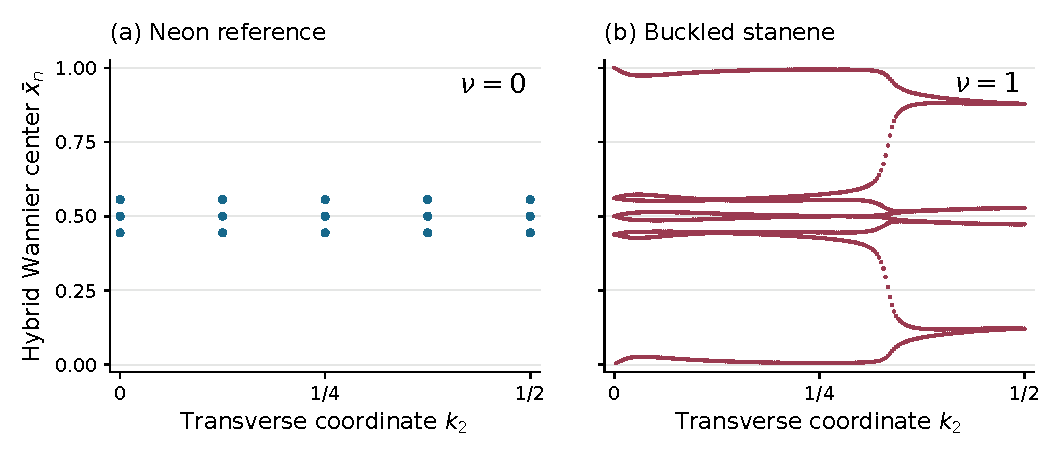
\includegraphics[width=\linewidth]{figures/wilson-centers.pdf}
 \caption{Wilson-loop test and demonstration calculations for
 (a) a periodic neon reference and
 (b) buckled stanene. Points are the computed hybrid Wannier centers in
 reduced units. Degenerate centers coincide. Each loop winds once along
 the first reciprocal coordinate, while the transverse coordinate spans
 $0\leq k_2\leq 1/2$ at $k_3=0$. The neon and stanene surfaces contain
 five and 193 loops, respectively, and yield $\nu=0$ and $\nu=1$.
 All eight occupied spinor centers are shown.}
 \label{fig:topology}
\end{figure}

\section{Crystalline representations and topological quantum chemistry}
\label{sec:tqc}
\subsection{Implemented inversion analysis}
An independently versioned native extension evaluates inversion
representations at time-reversal-invariant momenta (TRIM). This analysis
requires spatial inversion of the crystal, unlike the time-reversal
pairing used to reduce a scalar SCF mesh. The TRIM are diagonalized at
the converged SCF potential independently of the integration mesh,
without a Wannier90 execution or a Wannier fit. If
$T_{\mathcal I}(\bk)$ is the coefficient-space action of inversion,
including atom permutations, orbital parities and lattice phases, its
representation in the selected subspace is
\begin{equation}
 D_{\mathcal I}(\bk)=C^\dagger(\bk)S(\bk)
                   T_{\mathcal I}(\bk)C(\bk).
 \label{eq:topology-inversion}
\end{equation}
The overlap metric distinguishes the coefficient transformation
$T_{\mathcal I}$ from the covariant AO matrix of the inversion operator.
Character decomposition gives even and odd multiplicities without
assigning gauge-dependent labels to individual vectors within a mixed
degenerate eigenspace. For spinful time-reversal symmetry, the number of
odd occupied Kramers pairs yields the two-dimensional plane index or
the three-dimensional strong and weak Fu--Kane
indices~\cite{FuKane2007}, together with an inversion $z_4$ indicator
in three dimensions. An exact integer comparison with the analytic
inversion-subgroup elementary-band-representation (EBR) signatures also
tests membership in their integer lattice and the existence of a
nonnegative decomposition~\cite{Bradlyn2017,Po2017}. The implementation
uses inversion rather than a complete space-group EBR catalogue, and an
atomic-compatible signature does not establish trivial topology.
Metric, subspace, energy-commutator and time-reversal checks precede
classification. Additional parity calculations recover $\nu=0$ for
neon and $\nu=1$ for stanene. The separately versioned tests are described
in the Supporting Information and leave the retained Wilson spectra
unchanged.


\subsection{Little groups, nonsymmorphic phases, and spin}
The extension from inversion to general crystalline symmetry needs more
than a list of point rotations. Write a space-group operation as
$g=\{W_g|\tau_g\}$ in fractional direct coordinates, so that
$x\mapsto W_gx+\tau_g$. For cell matrix $A$, the Cartesian operation is
$R_g=AW_gA^{-1}$. Reciprocal fractional vectors transform with
$W_g^{-T}$, not in general with $W_g$. An antiunitary operation
$g\Theta$ additionally reverses $\bk$.

At a fixed fractional $\bk$, the little group contains operations
mapping $\bk$ to itself modulo a reciprocal vector. Choose one
representative per coset modulo integer translations of the cell.
Composition gives
\begin{equation}
 W_{gh}=W_gW_h,\qquad
 L(g,h)=\tau_g+W_g\tau_h-\tau_{gh}\in\mathbb Z^3 .
 \label{eq:coset-products}
\end{equation}
For spinors, the SU(2) lifts additionally give a sign $z(g,h)$.
The matrices acting in a fixed Bloch subspace must satisfy
\begin{equation}
 D_g\,{}^{a_g}\!D_h=\omega(g,h)D_{gh},\qquad
 \omega(g,h)=e^{-2\pi\ii\bk\cdot L(g,h)}z(g,h),
 \label{eq:projective-group}
\end{equation}
where $a_g=1$ denotes antiunitarity and
\({}^{1}\!D_h=\overline{D_h}\).
Physical $\Theta^2=-1$ contributes to the spin factor.
Associativity requires the twisted cocycle identity
\begin{equation}
 \omega(g,h)\omega(gh,j)
 ={}^{a_g}\!\omega(h,j)\,\omega(g,hj).
 \label{eq:cocycle}
\end{equation}
This distinguishes screw/glide operations from a point-group
approximation and double-valued representations from scalar ones
\cite{SpglibDefinitions,SpgrepFormulation}.

A conventional centered cell has distinct cosets with the same rotation
and different translations. Collapsing them by rotation alone loses
folded translation sectors. Conversely, character data calculated in
that conventional quotient cannot be matched blindly to a primitive-cell
EBR table. Both the cell transformation and representation convention
must be recorded.

\subsection{Metric sewing and degeneracies}
Let $T_g$ contain the atom/AO action, Bloch-image phases and spin action.
The sewing matrix between selected frames is
\begin{equation}
 B_g(\bk)=C^\dagger(g\bk)S(g\bk)
 T_g(\bk)\,{}^{a_g}\!C(\bk).
 \label{eq:sewing}
\end{equation}
For a closed selected subspace it is unitary and reconstructs the
transformed frame. Metric normalization, closure, and energy
compatibility must be checked before extracting characters.
Degeneracy is not resolved by labelling individual eigenvectors:
unitary rotations within a degenerate block are physically arbitrary.

For a unitary little group and a complete character table with the
same factor system, multiplicities follow from
\begin{equation}
 n_\alpha=\frac{1}{|G_{\bk}|}
 \sum_{g\in G_{\bk}}\overline{\chi_\alpha(g)}\,\chi(g).
 \label{eq:character-decomposition}
\end{equation}
The result must be a nonnegative integer, with consistent reconstructed
character and total dimension. Antiunitary operations require
corepresentation theory, not unmodified use of this character formula.
Characters alone also do not determine the sewing of directed Wilson
links between different k-points.

The native implementation constructs a complete projective character
table for the supplied unitary little group, rather than importing
standard-label tables. Actual GPW/GAPW Gaussian coefficient actions
include the atom permutation, AO rotation, cell-image phase and,
where requested, the post-SCF GTH spinor action. The selected band
sewing matrices are checked against Eq.~\eqref{eq:projective-group}
before characters are decomposed. Failed covariance or noninteger
multiplicities are rejected, not repaired by rotating eigenvectors
or rounding a defective representation.

\subsection{Antiunitary corepresentations}
Let the little group be $M=H\cup aH$, where $H$ is its unitary
subgroup. An irreducible projective character $\chi_\alpha$ of $H$
has antiunitary partner
\begin{equation}
 \chi_\alpha^a(h)=
 \frac{\omega(h,a)}{\omega(a,a^{-1}ha)}
 \overline{\chi_\alpha(a^{-1}ha)} .
 \label{eq:corep-partner}
\end{equation}
The Wigner indicator is~\cite{SpgrepCorepresentations}
\begin{equation}
 w_\alpha=\frac{1}{|H|}\sum_{b\in aH}
                  \omega(b,b)\chi_\alpha(b^2)\in\{+1,-1,0\}.
 \label{eq:wigner-corep}
\end{equation}
Type $+1$ retains one copy of the unitary irrep, type $-1$ requires
two copies, and type $0$ pairs two inequivalent partner irreps.
The native implementation determines these types and their integer
unitary restriction matrix. Odd type-$-1$ multiplicities or unequal
type-$0$ partner counts invalidate a selected band space.
Spin and nonsymmorphic phases enter the same factor system and cannot
be tested separately after those phases have been discarded.

These signs are neither topological indices nor antiunitary
eigenvalues. Type $+1$ does not exclude Kramers degeneracy: an
already multidimensional spin irrep can contain the required doublet
without additional doubling. At a generic centrosymmetric SOC point,
in contrast, the identity-only unitary subgroup may be doubled by
the combined inversion--time-reversal operation.
No canonical antiunitary eigenvector basis is assigned.
The electronic-structure path currently constructs the nonmagnetic
grey extension of the spatial group. The underlying algebra also
accepts supplied magnetic factor systems, but this is not a magnetic
space-group search or self-consistent noncollinear SOC calculation.

\subsection{Nonsymmorphic band compatibility on explicit segments}
For a directed connection from $\bk_a$ to $\bk_b+\bG$, define
$\mathbf d=\bk_b+\bG-\bk_a$. A segment symmetry must satisfy
\begin{equation}
 \sigma_g W_g^T\mathbf d=\mathbf d,\qquad
 \sigma_g=(-1)^{a_g},
 \label{eq:line-stabilizer}
\end{equation}
within the fractional-coordinate tolerance, not merely modulo a
reciprocal vector. Intersection of the endpoint little groups is
insufficient: ordinary time reversal can fix two TRIM endpoints
without preserving any interior point of their connecting segment.

To compare representations at the endpoints, remove the continuously
varying translational part using
\begin{equation}
 \eta_g(\bk)=e^{2\pi\ii\bk\cdot\tau_g},\qquad
 \bar\omega(g,h)=\eta_g\,{}^{a_g}\!\eta_h\,
                         \eta_{gh}^*\omega(g,h).
 \label{eq:line-rephasing}
\end{equation}
The conjugation for an antiunitary first factor is essential.
Both endpoints must produce the same rephased factor on the segment
subgroup. Its unitary projective characters provide a common basis
for integer endpoint-to-line branching matrices $B_a,B_b$.
With selected endpoint multiplicities $m_a,m_b$, compatibility requires
\begin{equation}
 B_a m_a=B_b m_b .
 \label{eq:line-compatibility}
\end{equation}
The destination rephasing uses $\bk_b+\bG$, not just $\bk_b$.
For example, a screw eigenvalue branch may exchange with another after
one reciprocal period. Ignoring $\bG$ would erase this monodromy.
Integer changes of coset representatives cancel between the
characters and the rephasing.

Endpoint corepresentations are restricted as whole representations.
If $R_a$ and $R_\ell$ give the unitary restrictions of endpoint and
line corepresentations, their branching $C_a$ satisfies
\begin{equation}
 R_\ell C_a=B_a R_a .
 \label{eq:corep-subduction}
\end{equation}
If the line has no antiunitary stabilizer, $B_aR_a$ instead describes
the branching into unitary line irreps. This retains endpoint partner
constraints even when time reversal is absent on the interior.
A spinful glide model illustrates the distinction: opposite glide
partners at Gamma become same-branch pairs at the boundary, preventing
an isolated two-band connection but allowing a four-band one.
For valid corepresentations, unitary and corepresentation line-count
compatibility are equivalent; the latter resolves the partner
structure rather than introducing a new invariant.

These operations are implemented on explicit NNKP or generated Wilson
links through \texttt{LITTLE\_GROUP\_COMPATIBILITY}, which implies
\texttt{LITTLE\_GROUP\_IRREPS}. Compatible endpoints do not prove a gap
between sampled points, a trivial Bloch bundle, or an atomic-band
decomposition. Automatic complete Brillouin-zone connectivity and
standard crystallographic irrep labels remain separate work.

\subsection{Site-induced atomic band representations}
The native induction kernel starts from a supplied fractional site $q$
and constructs its orbit $q_j=t_jq$ modulo integer translations.
Representatives $t_j$ are adjusted by lattice translations to reach the
chosen positions exactly. Localized orbitals carry irreps of the site
stabilizer; an antiunitary stabilizer instead requires the complete
corepresentations described above. Their unitary restriction characters
are denoted by $\chi_\alpha$.

For a unitary little-group operation $g$ that fixes site $j$ modulo
translations, set
\begin{equation}
 L_{gj}=W_gq_j+\tau_g-q_j\in\mathbb Z^3,\qquad
 h_j=t_j^{-1}\{I|-L_{gj}\}g t_j .
\end{equation}
The induced character is
\begin{equation}
 \chi^{\uparrow}_\alpha(g;\bk)=
 \sum_{j:\,gq_j=q_j\bmod\mathbb Z^3}
 e^{-2\pi\ii\bk\cdot L_{gj}}
 \frac{z(g,t_j)}{z(t_j,h_j)}\,
 {}^{a_{t_j}}\!\chi_\alpha(h_j).
 \label{eq:atomic-induction}
\end{equation}
This is the Bloch form of site induction~\cite{CanoBradlyn2021}, with
the spin factor in the same convention as Eq.~\eqref{eq:projective-group}.
Antiunitary orbit representatives conjugate the onsite character even
though $g$ itself is unitary. Omitting this conjugation loses complex
orbital partners.

The implementation retains conventional-cell centering cosets and keeps
each local representation column fixed across k points. Its band rank
is the orbit multiplicity times the local dimension. No full band
diagonalization or orbital gauge choice is needed to generate these
atomic reference characters. Validation compares their little-group
decompositions and segment restrictions with independent Cartesian
s/p/d orbital and spin traces. Site induction alone neither enumerates
all Wyckoff positions nor establishes that an induced representation
is elementary.

\subsection{Generating site-symmetry families}
The possible atomic reference positions need not be occupied by atoms
in the input structure. A separate geometric kernel obtains them from
the complete supplied space group. For each operation it solves
\begin{equation}
 (W_g-I)q=-\tau_g\pmod{\mathbb Z^3}
\end{equation}
and closes the resulting connected fixed sets under nonempty
intersection. Saturating the integer row lattice yields primitive
normals $B$ for each connected affine torus,
\begin{equation}
 Bq=c\pmod{\mathbb Z^r},\qquad d=3-r.
\end{equation}
Distinct components are retained: for example, $2q_x=0\pmod1$
contains both $q_x=0$ and $q_x=1/2$. Integer right-hand sides are
enumerated from the bounds of the unit cube rather than by sampling
a coordinate mesh. Subsequent space-group equivalence identifies the
families, and a generic representative is checked against its entire
site stabilizer.

Closure containment supplies specialization relations between families.
A site group is maximal when its family has no higher-symmetry
specialization. This provides the geometric input to site induction,
but does not replace the representation-level elementarity tests needed
for an EBR catalogue. The construction retains the supplied cell and
origin conventions and does not assign standard Wyckoff letters.

\subsection{Atomic signature matrices on explicit reciprocal sets}
Combining the generated sites with the induction kernel gives a native
integer signature matrix for a supplied reciprocal set $\mathcal K$,
\begin{equation}
 A_{(\bk,\beta),(q,\alpha)}
 =n_{\beta}\!\left[\chi^{\uparrow}_{q,\alpha}(\cdot;\bk)\right],
 \qquad \bk\in\mathcal K .
\end{equation}
The column $(q,\alpha)$ retains one Wyckoff-family representative and
one onsite irrep or corepresentation at every point. Rows use unitary
irreps unless the little group has an antiunitary coset; in that case
they count complete corepresentations after checking the required
unitary partner multiplicities. Consequently,
\begin{equation}
 \sum_\beta d_{\bk\beta} A_{(\bk,\beta),(q,\alpha)}
 =N_{q\alpha}
\end{equation}
is the same physical band rank for every $\bk$. Counts are not generally
numbers of Kramers pairs: corepresentation dimensions and pairing types
are retained explicitly.

The implementation preserves all sites, including nonmaximal ones,
and does not identify columns merely because their sampled signatures
coincide. An incoming unitary character vector can be decomposed in
the same row basis after matching its operation indices, provided it
uses the same spin/Bloch convention. This algebraic check does not replace
Hamiltonian covariance or selected-subspace closure for actual Gaussian
states. The matrix remains a redundant atomic reference for the
explicit set $\mathcal K$, not an automatically complete EBR matrix:
reciprocal-stratum completeness and representation elementarity remain
separate from the integer decomposition of this supplied matrix.

\subsection{Exact signed and nonnegative signature decompositions}
For an integer signature matrix $A\in\mathbb Z^{m\times n}$, the native
integer kernel constructs a Smith form~\cite{CanoBradlyn2021},
\begin{equation}
 UAV=D,\qquad
 D=\operatorname{diag}(d_1,\ldots,d_r,0,\ldots),\qquad
 d_i>0,\quad d_i\mid d_{i+1},
\end{equation}
where $U$ and $V$ are unimodular integer matrices. With $c=Ub$,
the equation $Ax=b$ has an integer solution precisely when
\begin{equation}
 c_i=0\quad(i>r),\qquad c_i\equiv0\pmod{d_i}\quad(i\leq r).
\end{equation}
A witness is obtained as $x=Vy$, with $y_i=c_i/d_i$ for $i\leq r$
and zero free components. The implementation checks both $UAV=D$
and $Ax=b$ using bounded 64-bit integer arithmetic. Rank decisions
do not use floating-point thresholds. Growth beyond the arithmetic
bound or exhaustion of the factorization work limit returns an
unresolved status, not a negative membership decision.

For the nonnegative signature matrices used here, the stronger condition
$Ax=b$, $x\in\mathbb Z_{\geq0}^n$, is tested separately. At a search
node with residual $b'\geq0$, a nonzero column $j$ has the finite bound
\begin{equation}
 0\leq x_j\leq
 \min_{i:A_{ij}>0}\left\lfloor\frac{b'_i}{A_{ij}}\right\rfloor.
\end{equation}
Row-wise gcds of the remaining columns and their zero supports prune
the complete enumeration; zero columns can be set to zero. Every
accepted witness is checked exactly. A caller-specified node budget
bounds the potentially exponential search. An exhausted budget is
explicitly undecided and must not be interpreted as absence of an
atomic decomposition.

These are decisions about the supplied columns and sampled rows.
The Smith divisors of an incomplete reciprocal sample are not, by
themselves, the space group's symmetry-indicator group. Nonnegative
membership likewise does not prove triviality of a Bloch bundle.
The integer routines do not add an automatic general-classification
input mode or replace spectral isolation and compatibility checks.

\subsection{Band representations and limits of indicators}
Elementary band representations (EBRs) provide the indecomposable
building blocks of atomic band representations. Restricting them to
little groups yields a vector of irrep multiplicities. Compatibility
relations constrain the vectors that can connect along high-symmetry
lines. A candidate symmetry vector $n$ can be compared with an integer
matrix of EBR signatures,
\begin{equation}
 E q=n .
 \label{eq:ebr-system}
\end{equation}
Integer solvability, nonnegative solvability, and compatibility
constraints are different questions. A symmetry indicator is a
quotient of compatible representation data by atomic data; it can
miss topology invisible to those symmetry eigenvalues
\cite{Bradlyn2017,Po2017}.
An atomic-compatible signature is not proof of a trivial Bloch bundle.
A signed-only decomposition is not, without additional information,
a complete diagnosis of fragile topology.

The implemented EBR-signature classifier still uses the inversion
subgroup and its analytic atomic signatures. The general native
little-group/corepresentation, explicit-segment, Wyckoff-family and site-induction
machinery supplies additional representation data, not a complete
all-space-group classification. Conventional-to-primitive matching,
standard labels, complete connectivity and a validated catalogue with
elementarity checks are still required. Algebra tests over all ordinary
space groups must not be presented as a completed classification
of all their materials.

\section{Parameter-space topology and phasons}
\label{sec:phasons}
A separate native postprocessor, \texttt{topology\_phasons}, extends the
overlap construction to closed two- or four-parameter families, including
periodic atomic displacements (phasons) combined with reciprocal
coordinates. It reads \texttt{STATE\_EXPORT} snapshots and evaluates
$M_{ab}=C_a^\dagger O_{ab}C_b$, where $O_{ab}$ includes the Gaussian
centers of both geometries, periodic images, and Bloch and boundary-sewing
phases. Polar-unitary links give $C_1$ from determinant plaquette
phases~\cite{Fukui2005} and a four-parameter $C_2$ estimate from full
non-Abelian plaquette logarithms~\cite{MocholGrzelak2019}. Here $C_2$
denotes the second Chern character pairing, not generally the second
Chern class. The postprocessor requires neither Python, Z2Pack, nor
Wannier90 at runtime. It operates on fixed-cell, fixed-rank families with
explicit physical endpoint identifications. The Supporting Information
gives its separate development version, discretization, and model and
Gaussian-snapshot tests. These tests complement the material examples
below without changing their Hamiltonians, sampling, or results.


For a discrete parameter family, let $Q_\mu(x)$ denote the polar link
from $x$ to $x+\hat\mu$. An oriented plaquette is
\begin{equation}
 P_{\mu\nu}(x)=Q_\mu(x)Q_\nu(x+\hat\mu)
 Q_\mu^\dagger(x+\hat\nu)Q_\nu^\dagger(x).
\end{equation}
With the implemented directed-overlap convention,
$C_1^{\mathrm{mesh}}=-(2\pi)^{-1}\sum_x\arg\det P_{12}(x)$.
For four parameters write $F_{\mu\nu}(x)=\log P_{\mu\nu}(x)$
using the principal matrix logarithm. The non-Abelian estimator is
\begin{equation}
 C_2^{\mathrm{mesh}}=-\frac{1}{4\pi^2}\sum_x
 \Re\Tr\!\left[F_{12}F_{34}-F_{13}F_{24}+F_{14}F_{23}\right](x).
 \label{eq:phason-c2}
\end{equation}
The logarithms already include the discrete plaquette area.
Mesh refinement, physical endpoint identifications, and a fixed isolated
rank are essential. Coefficient arrays from different geometries
cannot be contracted without cross-geometry AO overlaps.
The numerical value is retained before rounding, and a sampled gap
does not certify isolation between sampled geometries.

\section{Spectral localizers in finite and periodic systems}
\label{sec:localizer}
\subsection{Energy-position tuples and Clifford structure}
A spectral localizer combines operators associated with several
observables into one self-adjoint matrix. For two positions and a
Hamiltonian, Pauli matrices provide a Clifford representation.
In an orthonormal space define
\begin{equation}
 \widetilde L=
 (\widetilde H-EI)\otimes\sigma_z+
 \kappa(\widetilde X-xI)\otimes\sigma_x+
 \kappa(\widetilde Y-yI)\otimes\sigma_y ,
 \label{eq:clifford-localizer}
\end{equation}
up to the explicitly fixed tensor ordering.
The parameter $\kappa>0$ has units of energy/length.
It balances energy and position resolution rather than correcting
the Hamiltonian. The connection between a localizer signature and
an even index pairing holds under appropriate locality, gap, and
finite-volume bounds \cite{LoringSchulzBaldes2020}.
Those hypotheses remain relevant when interpreting a finite Gaussian model.

In auxiliary-index-first ordering the covariant AO matrix is
\begin{equation}
 L=
 \begin{pmatrix}
 H-ES & \kappa[(X-xS)-\ii(Y-yS)]\\
 \kappa[(X-xS)+\ii(Y-yS)] & -(H-ES)
 \end{pmatrix},\qquad
 B=\begin{pmatrix}S&0\\0&S\end{pmatrix}.
 \label{eq:covariant-localizer}
\end{equation}
For SOC, $H$ and $S$ here denote the physical spinor matrices.
Auxiliary doubling is separate from spin, so the localizer dimension
is four times the scalar AO count. All AO directions are retained:
there is no hidden occupied-space projection or automatic removal
of nearly dependent basis functions.

\subsection{Index, metric gap, and stability}
For class A define
\begin{equation}
 \nu_A=\frac12\Sig(L)=\frac12(n_+-n_-),\qquad
 \mu=\min_j|\lambda_j|,\quad Lv_j=\lambda_j Bv_j .
 \label{eq:index-gap}
\end{equation}
Signature is invariant under nonsingular congruence, whereas ordinary
eigenvalues of a covariant AO matrix are not.
Inertia can therefore be evaluated directly from $L$, but the
protection gap must retain $B$. Equivalently, $\mu$ is the smallest
absolute eigenvalue of $B^{-1/2}LB^{-1/2}$; this identity does not
require forming that dense matrix.

At fixed metric, the index cannot change under a perturbation satisfying
\begin{equation}
 \|B^{-1/2}\delta L B^{-1/2}\|<\mu .
 \label{eq:localizer-stability}
\end{equation}
This finite-matrix statement gives local protection an operational
meaning. If the metric changes, the corresponding orthonormalized
problems must be compared, including the effect of $\delta B$.
An unresolved near-zero gap yields an \emph{unresolved} index,
not evidence for trivial topology.

Moving the query and coordinate operators together, shifting the
Hamiltonian and query energy together, or changing AO basis must
leave the generalized gap unchanged. Reversing the oriented plane
reverses the class A sign. Model comparisons establish the sign
convention before applying it to a material.

\subsection{Inertia and gap require different calculations}
A pivoted Hermitian factorization has the form
\begin{equation}
 P^\dagger LP=\mathcal L D\mathcal L^\dagger .
 \label{eq:ldl}
\end{equation}
Here $\mathcal L$ is unit lower triangular and $D$ contains
$1\times1$ and $2\times2$ blocks.
Sylvester's law transfers the inertia from $L$ to $D$.
For a Hermitian block,
\[
 D_b=\begin{pmatrix}a&b\\\overline b&d\end{pmatrix},\qquad
 \lambda_\pm=\frac{a+d}{2}
 \pm\sqrt{\left(\frac{a-d}{2}\right)^2+|b|^2}.
\]
Stable evaluation must retain scaling and both signs.
A zero-diagonal block with $b\ne0$ has one positive and one negative
direction; counting its diagonal entries is wrong.
The dense reference uses LAPACK \texttt{ZHETRF}, with \texttt{DSYTRF}
for exactly real matrices \cite{LapackLDL}. A small imaginary part is
not discarded to select real arithmetic.

Pivot magnitudes are not generalized gaps. For $\sigma>0$,
shifted inertia counts satisfy, away from singular endpoints,
\begin{equation}
 \begin{split}
 n_-(L-\sigma B)-n_-(L)&=\#\{j:0<\lambda_j<\sigma\},\\
 n_-(L)-n_-(L+\sigma B)&=\#\{j:-\sigma<\lambda_j<0\}.
 \end{split}
 \label{eq:gap-inertia}
\end{equation}
These counts bracket the nearest positive or negative generalized
eigenvalue. Factorization failure or an ambiguous endpoint must not
be treated as a successful certificate. The reported bounds are
finite-precision numerical brackets, not interval-arithmetic guarantees.

\subsection{Pfaffian orientation and physical time reversal}
For a real skew-symmetric matrix $A$ of even order,
$\det A=\Pf(A)^2$: the determinant loses the Pfaffian sign.
Moreover, $\Pf(P^TAP)=\det(P)\Pf(A)$.
An odd simultaneous row/column permutation reverses that sign
without changing the determinant.
Ordinary inertia cannot replace a skew factorization with explicit
permutation bookkeeping.

For spinful time reversal with $\Theta^2=-1$, the localizer has
a real skew representation \cite{DollSchulzBaldes2021,Wong2026}.
In auxiliary/spin/AO ordering, let $C=J_{\mathrm{aux}}\otimes J$
and $Q=(I-\ii C)/\sqrt2$. The symmetry relations imply that
\begin{equation}
 A=\ii Q^\dagger LQ
 \label{eq:aii-skew}
\end{equation}
is real and skew-symmetric. Both properties are checked numerically,
with residuals small relative to the independently resolved metric
gap. An arbitrary complex AO basis change also transforms time
reversal; keeping $J$ fixed would generally be inconsistent.

Let $A_0$ be the corresponding transform of
$L_0=\operatorname{diag}(S,-S)$. The reference-calibrated index is
\begin{equation}
 (-1)^{\nu_{\mathrm{AII}}}
 =\operatorname{sgn}\Pf(A)\,
  \operatorname{sgn}\Pf(A_0).
 \label{eq:pfaffian-index}
\end{equation}
Both factors use the same ordering and orientation.
The dense algorithm accumulates signs rather than an overflowing
Pfaffian product. This is a time-reversal local index,
not an inversion-parity test.

The native sparse skew factorization implements a separate numerical
task from symmetric inertia. It retains a distributed Schur complement
and oriented $2\times2$ pivots, accumulating the pivot signs and the
parity of their permutations. The transformation in
Eq.~\eqref{eq:aii-skew} is assembled by distributed addition of
coordinate entries rather than by gathering a dense matrix.
Independent right-hand sides test the retained factors against the
assembled matrix. The discarded symmetric and imaginary parts are
bounded relative to the independently resolved metric gap before
an index is accepted. This calculation requires neither MUMPS nor
Tacho. The optional Tacho comparison implements the same separate
skew-Pfaffian task \cite{Wong2026}, but its factorization resides on
one rank and is not an MPI-distributed Pfaffian solver.
The motivating photonic and aperiodic examples
\cite{Dixon2023,Wong2026} provide methodological context, not
first-principles material validation for the CP2K path.

\subsection{Finite three-dimensional class AII}
For three Cartesian positions, the finite AII construction uses
a real determinant rather than the two-dimensional Pfaffian
\cite{Loring2015}. In auxiliary-index-first ordering, define
\begin{equation}
 \begin{split}
 A_3&=I_2\otimes(H-ES)
       -\ii\kappa\sum_{j=1}^{3}\sigma_j\otimes(X_j-x_jS),\\
 B_3&=I_2\otimes S,\qquad
 L_3=\begin{pmatrix}0&A_3\\A_3^\dagger&0\end{pmatrix},\qquad
 \mathcal B_3=\operatorname{diag}(B_3,B_3).
 \end{split}
 \label{eq:finite-three-dimensional-localizer}
\end{equation}
Here $X_j$ are the covariant Cartesian moments, $x_j$ are the
query coordinates, and the Pauli matrices $\sigma_j$ act only
in the auxiliary space. The physical-spin Hamiltonian, metric
and all three positions must obey the fixed fermionic
time-reversal representation. With $C=J_{\mathrm{aux}}\otimes J$
and $Q=(I-\ii C)/\sqrt2$, the chiral block
$R_3=Q^\dagger A_3Q$ is real but need not be symmetric.
For a resolved gap, the local index is
\begin{equation}
 \nu_3=\frac{1-\operatorname{sgn}\det R_3}{2},\qquad
 \mu_3=\min_\ell|\lambda_\ell|,\qquad
 L_3v_\ell=\lambda_\ell\mathcal B_3v_\ell .
 \label{eq:finite-three-dimensional-index}
\end{equation}
Equivalently, $\mu_3$ is the smallest singular value of
$B_3^{-1/2}A_3B_3^{-1/2}$. Nonsingular AO congruences
multiply the determinant by a positive factor and preserve
the metric gap. A basis change must also preserve or
consistently transform the time-reversal representation.

The dense implementation accumulates triangular-pivot and
permutation signs without forming a determinant product.
The factor reconstruction residual and a rounding allowance
are compared with the independently calculated metric gap.
If excessive pivot growth prevents acceptance of the triangular
factorization, a Householder factorization supplies orthogonal
and upper triangular factors instead. The determinant sign
includes every nonidentity reflection. The discarded imaginary
part of $R_3$ is included in the perturbation budget, and an
unresolved calculation returns no topological label.

The Hermitian pencil has order eight times the scalar AO count.
Its current solver is a dense reference, including
GPW/GAPW and post-SCF GTH SOC. The periodic extension is given
below, while a sparse three-dimensional solver is not provided.
This strong local index is
not a collection of weak or two-dimensional slice indices.
Agreement with a bulk invariant requires separate volume,
basis and scale convergence. The Supporting Information
includes an explicit finite-box counterexample to automatic
identification with the bulk parity.

\subsection{Periodic positions and the torus construction}
A Cartesian coordinate truncated to a primitive cell is discontinuous
at the periodic seam. Using it in the open-boundary localizer is not
a periodic formulation.
Instead, analytic periodic functions are used \cite{Doll2025}.
For analysis-torus reciprocal vectors $\bG_j$ and
$\phi_j=\bG_j\cdot\br_0$, define
\begin{equation}
 \begin{split}
 C_j&=\langle\phi_\mu|\cos(\bG_j\cdot\br-\phi_j)|\phi_\nu\rangle,\\
 T_j&=\langle\phi_\mu|\sin(\bG_j\cdot\br-\phi_j)|\phi_\nu\rangle .
 \end{split}
\end{equation}
In the implemented orientation,
\begin{equation}
 L_{\mathrm{per}}=
 \begin{pmatrix}
 H-ES-\eta(2S-C_1-C_2)&\eta(T_1-\ii T_2)\\
 \eta(T_1+\ii T_2)&-H+ES+\eta(2S-C_1-C_2)
 \end{pmatrix}.
 \label{eq:periodic-localizer}
\end{equation}
The energy scale $\eta$ is distinct from $\kappa$, and the metric
remains $\operatorname{diag}(S,S)$.
An overall sign and auxiliary-space conjugation relative to the
cited periodic construction make its orientation consistent with
the finite localizer used here.

The trigonometric operators are integrated directly, not evaluated
as matrix functions of finite projected Cartesian positions.
Projection need not preserve either exact unitarity of exponentials
or their commutativity. The theorem for a gapped finite-range lattice
Hamiltonian therefore does not automatically become a theorem for
an arbitrary Gaussian projection.
The output is an AO-torus diagnostic requiring independent
basis-, torus-, and scale-converged material checks.

Explicit analysis k-points describe the enlarged torus through its
complete mesh. Periodic exponentials shift between mesh sectors,
so their cross-k links must be retained.
A symmetry-reduced SCF can supply the potential, but scalar SCF
weights cannot replace the full torus operator.
For three periodic directions, the corresponding chiral block is
\begin{equation}
 \begin{split}
 A_{3,\mathrm{per}}={}&I_2\otimes
   \left[H-ES-\eta\left(3S-\sum_{j=1}^3C_j\right)\right]\\
 &-\ii\eta\sum_{j=1}^3\sigma_j\otimes T_j .
 \end{split}
 \label{eq:periodic-three-dimensional-localizer}
\end{equation}
The phase-shifted $C_j,T_j$ are the analytic AO integrals defined
above, and $\eta>0$ has energy units. Replacing $A_3$ by
$A_{3,\mathrm{per}}$ in Eqs.~\eqref{eq:finite-three-dimensional-localizer}
and \eqref{eq:finite-three-dimensional-index} gives the Hermitian
metric pencil, real determinant sign and gap. In this orientation
the chiral block is an energy-scaled adjoint of the odd-dimensional
periodic construction of Ref.~\cite{Doll2025}. Taking the adjoint
preserves the sign of its real determinant.
The native three-dimensional path uses all three torus directions
with fully periodic cell and Poisson boundaries, fermionic time
reversal and the dense AII solver. Its finite-AO validation includes
skew cells, origin periodicity and GPW/GAPW comparisons. It is not
a sparse implementation or a bulk-convergence certificate.

Spectral flattening provides a separate way to examine the large
bandwidth-to-gap ratio of a DFT Hamiltonian. For positive $S$ and
$E$ in a resolved electronic gap, define
\begin{equation}
 \begin{aligned}
 F_E&=\Delta S\,\operatorname{sign}\!\left[S^{-1}(H-ES)\right]\\
 &=\Delta S^{1/2}\operatorname{sign}\!\left[S^{-1/2}(H-ES)S^{-1/2}\right]S^{1/2},
 \qquad \Delta>0 .
 \end{aligned}
 \label{eq:covariant-flattening}
\end{equation}
This covariant Hermitian operator retains the occupied projector
and replaces generalized band energies by $\pm\Delta$.
The dispersion-reduction argument for periodic localizers motivates
this control \cite{Doll2025}. It does not equate a flattened
finite-volume localizer with the original one: the localizer gap
can close during flattening even when the electronic gap stays open.
An exact sign is also generally longer ranged than $H$.
Consequently, the material tests in the Supporting Information
are distinguished from a proof of the finite-range theorem's
hypotheses and from the native unflattened calculation.

The optional \texttt{SPECTRAL\_FLATTENING} path evaluates
Eq.~\eqref{eq:covariant-flattening} for finite systems with
distributed DBCSR metric inversion and matrix-sign iterations.
Before those iterations,
the original positive metric and the distance of $E$ to the
generalized spectrum of $(H,S)$ are checked by dense diagonalization
or shifted MUMPS factorizations. An unresolved electronic gap is
rejected rather than enlarged by flattening. This precondition is
distinct from the gap of the final localizer. The transformed
Hamiltonian is reused across position and scale queries at fixed
$E$; the SCF Hamiltonian and Gaussian coordinate operators remain
unchanged. The option is off by default. The distributed inverse
and exact-sign approximation can increase fill-in, so this path
does not imply linear scaling.

For a translation-invariant periodic AO torus, the same sign can
instead be evaluated in complete primitive Bloch blocks.
The implementation verifies translation covariance of the entire
Hamiltonian and metric before extracting a representative block row.
It distributes full generalized Bloch eigensystems over MPI ranks,
forms $F_E(k)=\Delta S(k)C(k)\operatorname{sign}(\epsilon_k-E)
C(k)^\dagger S(k)$, and Fourier-transforms back to the original
distributed spin/cell/atom order. The metric bounds and electronic
gap refer to the union of all sampled Bloch spectra. No bands are
discarded and no independent localizer is assigned to a single
k-point. This avoids a whole-torus eigensystem or sign iteration
for the flattening step; it does not remove the final localizer
solve or its possible fill-in.

\subsection{Connection to the quadratic pseudospectrum}
For Hermitian operators $A_j$ and anticommuting Hermitian Clifford
matrices $\gamma_j$, squaring $L=\sum_jA_j\otimes\gamma_j$ gives
\begin{equation}
 L^2=\left(\sum_j A_j^2\right)\otimes I+
 \sum_{j<l}[A_j,A_l]\otimes\gamma_j\gamma_l .
 \label{eq:clifford-square}
\end{equation}
The first term measures simultaneous approximate localization;
the second retains noncommutativity.
The quadratic gap and localizer gap are related, but not
interchangeable. In an AO basis each projected product must
include the metric, or be evaluated after orthonormalization.

\section{Quadratic pseudospectrum and localized approximate states}
\label{sec:quadratic}
The quadratic pseudospectrum asks for a normalized state that minimizes
the combined residual of incompatible observables \cite{Cerjan2023}.
For a query $(E,\bm x)$, set $A_0=H-ES$, $A_j=X_j-x_jS$,
$w_0=1$, and $w_j=\kappa$ for $j=1,2,3$. The AO problem is
\begin{equation}
 Qc=\lambda Sc,\qquad
 Q=\sum_{j=0}^3 w_j^2 A_j^\dagger S^{-1}A_j,\qquad c^\dagger Sc=1 .
 \label{eq:quadratic}
\end{equation}
The minimum $\sqrt{\lambda}$ is the quadratic gap.
Its eigenvector is a joint approximate state, and several low
eigenpairs can describe a localized subspace.
The separated residuals are
\begin{equation}
 \begin{split}
 \delta E^2&=(A_0c)^\dagger S^{-1}(A_0c),\\
 \delta x_j^2&=(A_jc)^\dagger S^{-1}(A_jc),\\
 \lambda&=\delta E^2+\kappa^2\sum_j\delta x_j^2 .
 \end{split}
 \label{eq:quadratic-residuals}
\end{equation}
Expectations $c^\dagger Hc$ and $c^\dagger X_jc$ distinguish bias from
spread around the query. These states need not be eigenstates of $H$.
Within degenerate minimizing spaces, projectors or subspace observables
must be compared instead of individual coefficients.

Equation~\eqref{eq:quadratic} is positive semidefinite and covariant
under Eq.~\eqref{eq:basis-change}. Ordinary matrix products without
metric solutions would destroy that invariance.
The position residual concerns the projected position:
$X_jS^{-1}X_j$ is not an independently integrated continuum
$\langle r_j^2\rangle$. Small bases can underestimate continuum
localization errors even when the eigenproblem is solved accurately.

The dense reference uses a complete orthonormalized space.
The iterative path applies $Q$ without forming it: multiply by
$A_j$, solve with $S$, multiply by $A_j^\dagger$, and accumulate.
This avoids fill-in from explicitly squaring sparse matrices.
A complex block Rayleigh--Ritz iteration, double metric
reorthogonalization, and thick restarts address clustered low states.
The residual
\[
 \|Qc-\lambda Sc\|_{S^{-1}}
 \leq\epsilon_{\mathrm{eig}}\max(1,|\lambda|)
\]
checks an eigenpair in atomic units; it does not independently prove
that no lower state was missed.

Reusable MUMPS factors avoid forming $S^{-1}$, but the present
trial vectors and multiple-right-hand-side communication are not
fully distributed. Output includes separated residuals,
expectations, and optional complex AO coefficients.
The finite analysis covers isolated GPW/GAPW systems and post-SCF
GTH SOC. A small quadratic gap is a localization diagnostic,
not a Chern or $\mathbb Z_2$ index.

\subsection{Periodic joint localization on an AO torus}
The periodic formulation replaces the unbounded position by paired
trigonometric coordinates on a Born--von Karman torus. For cell
matrix $h$ and a full Gamma-centered $N_1\times N_2\times N_3$
property mesh, define, for each periodic lattice direction $j$,
\begin{equation}
 \begin{split}
 g_j&=\frac{2\pi}{N_j}(h^{-1})_{j,:},\qquad r_j=|g_j|^{-1},\\
 C_j&=\langle\cos(g_j\cdot r)\rangle_{\rm AO},\qquad
 D_j=\langle\sin(g_j\cdot r)\rangle_{\rm AO}.
 \end{split}
 \label{eq:quadratic-torus}
\end{equation}
These covariant matrices are assembled from the same ordered
Berry integrals and real-cell images as the periodic localizer.
For query $x$, replace each Cartesian observable in
Eq.~\eqref{eq:quadratic} by the two shifted operators
$C_j-\cos(g_j\cdot x)S$ and $D_j-\sin(g_j\cdot x)S$, both
weighted by $\kappa r_j$. With their dimensionless residuals
$\delta C_j$ and $\delta D_j$, the resulting problem satisfies
\begin{equation}
 \lambda=\delta E^2+\kappa^2\sum_{j\ \mathrm{periodic}}
 \delta\ell_j^2,\qquad
 \delta\ell_j=r_j\sqrt{\delta C_j^2+\delta D_j^2}.
 \label{eq:quadratic-chord}
\end{equation}
The length-valued chord residual is invariant under shifting the
query by a torus lattice vector. For skew cells this is a specified
reciprocal-coordinate metric, not an isotropic Cartesian variance;
changing the primitive-lattice basis can change that metric.
Finite AO projection also means that $C_j+iD_j$ need not be exactly
unitary. We do not replace it by a polar-unitarized operator.

The \texttt{FORMULATION PERIODIC} path uses the complete torus AO
space at the frozen SCF potential, independently of SCF symmetry
weights or reconstructed occupied MOs. It therefore accepts a
symmetry-reduced SCF calculation without claiming an irreducible
property eigensolver. One, two or three periodic directions are
supported; open directions are not localized by this formulation.
Output reports chord residuals and mean cosines/sines rather than
ambiguous Cartesian mean positions. Dense and DBCSR/MUMPS solvers
and the restricted post-SCF GTH-SOC construction share this tuple
of Hermitian operators. Translation-operator band unfolding is a
different joint-eigenvector problem and is not implemented here.

Small GPW/GAPW He and GTH-SOC Ne checks give serial-dense versus
two-rank-iterative gaps agreeing within $6\times10^{-15}$ hartree;
the maximum iterative eigenpair residual is
$6.7\times10^{-11}$ hartree$^2$. The He primitive-mesh and separately
converged Gamma-supercell gaps differ by less than $10^{-9}$ hartree.
Query wrapping, rigid cell rotation and equivalent SCF mesh schemes
provide additional consistency checks. Settings and limitations
are given in the Supporting Information; these are numerical
integration tests, not converged material localization predictions.

\section{Materials-discovery applications and demonstrative tests}
\label{sec:applications}
\subsection{Hybrid-functional topological materials databases}
TopoHSE-DB provides an application example of electronic-structure-based
topological classification at database scale
\cite{Mirhosseini2026TopoHSE}. Mirhosseini, Elcoro, Kn\"upfer and
K\"uhne combine consistently relaxed nonmagnetic crystal structures,
PBE and screened-hybrid HSE06 electronic structures, and topological
quantum chemistry. Comparing the resulting labels exposes the
sensitivity of a symmetry-based classification to the underlying
exchange--correlation approximation. A converged integer or symmetry
label is therefore not, by itself, evidence that the electronic
Hamiltonian has been described accurately.

The original database workflow uses VASP, VASP2Trace, and
CheckTopologicalMat. It is cited here as a materials-discovery
application and a source of future comparison cases, not as a
calculation performed with the new CP2K topology routines.
Connecting such a workflow to CP2K requires equivalent electronic
structure and symmetry conventions as well as the general little-group,
compatibility-relation, and EBR machinery discussed in
Section~\ref{sec:tqc}. The currently implemented inversion analysis
does not yet reproduce the database's full classification workflow.

\subsection{Generative--predictive discovery of candidate materials}
The submitted study by Brocai, K\"uhne, Kn\"upfer and Mirhosseini,
\emph{Generative--predictive models enable the discovery of topological
materials}, provides a complementary application
\cite{Brocai2026Discovery}. It couples topology-conditioned crystal
generation to a predictive filter using a shared pretrained
representation, followed by hybrid-functional electronic-structure
and TQC analysis. The submitted manuscript reports 1,033 successfully
calculated hybrid-functional band structures; 629 receive an unambiguous
classification and 523 are classified as topological. The corresponding
83.15\% rate applies to the classified subset, whereas the confirmed
yield across all 1,033 calculated cases is 50.6\%. The 404 unresolved
classifications must not be silently counted as either trivial or
topological.

These results, obtained with the study's VASP-based workflow, illustrate
the demand for reliable post-processing and explicit failure diagnostics.
They also motivate subsequent, distinct questions: Wilson spectra can
probe isolated band subspaces, Kubo calculations can address transport
at specified temperature and dissipation, and localizers can investigate
finite, defective, or disordered realizations of selected candidates.
These are prospective CP2K follow-up applications, not calculations
already completed for the reported candidate set. A TQC label alone
does not supply a conductivity or a localizer protection gap.

\subsection{Small calculations as tests and demonstrations}
The smaller calculations in this paper and the companion k-point
study serve a different purpose \cite{KpointCompanion2026}.
They provide transparent tests and demonstrations of individual
algorithmic steps, not a second materials-discovery survey.
Table~\ref{tab:demonstration-roles} states the role of each set.
\begin{table}[htbp]
\centering\small
\begin{tabular}{L{0.27\linewidth}L{0.59\linewidth}}
\toprule
Calculation set & Demonstration and test objective\\
\midrule
Si and Al, companion k-point study &
Quadrature dependence and equivalent full-grid, time-reversal,
K290, and SPGLIB representations. At fixed $4^3$ sampling,
64 eigensystems reduce to four with atomic symmetry.\\
Periodic neon and buckled stanene &
Trivial and nontrivial Wilson-loop examples, with $\nu=0$ and
$\nu=1$, respectively; comparison of native and external analyses.\\
Ne/SOC, Bi$_2$/SOC, and diamond/SOC &
Primitive-mesh versus supercell and reduced versus full-property-grid
checks of the metric, Hamiltonian, and current operators.\\
Analytic localizer models and small GPW/GAPW systems &
Known indices, gap closings, basis covariance, and dense/sparse
solver consistency; quadratic-state residual and subspace checks.\\
\bottomrule
\end{tabular}
\caption{Test and demonstration calculations, distinct from the
materials-discovery applications cited above. The Si/Al results are
retained from the companion study, not rerun or reassigned to the
new topology implementation.}
\label{tab:demonstration-roles}
\end{table}

For Si and Al, the largest fixed-mesh cell-energy or electronic-free-energy
difference among the compared representations is
$1.4\times10^{-12}$ hartree. This tests representation equivalence,
not complete basis or k-point convergence. In particular, the Al
free energy still changes by 10.721 meV per atom between the
$6^3$ and $8^3$ meshes. Likewise, agreement between Wilson analyses
using the same overlap matrices tests the analysis stage, while
independent operator identities test the AO construction.
The quantitative checks in Section~\ref{sec:validation} and the
Supporting Information retain these distinctions and their original
calculation provenance.

\section{Implementation, validation, and development boundaries}
\label{sec:validation}
\subsection{Shared operators and optional numerical backends}
The finite-system property paths share full AO Hamiltonians, overlap,
analytic positions, and optional GTH-SOC blocks.
DBCSR supplies distributed block storage and matrix products
\cite{Borstnik2014}. Localizer assembly retains the union of the
operator sparsity patterns without additional dropping.
DBCSR is not itself a general pivoted indefinite factorization or
Pfaffian solver.

The dense LAPACK path is the small-system reference. MUMPS supplies
distributed symmetric-indefinite factorizations and reusable metric
solutions \cite{MumpsGuide}. Complex Hermitian matrices are realified:
\begin{equation}
 \mathcal R(A)=
 \begin{pmatrix}\Re A&-\Im A\\\Im A&\Re A\end{pmatrix}.
\end{equation}
Each eigenvalue is duplicated, so inertia-based formulas compensate
for that duplication. A positive metric is checked separately from
the indefinite localizer. Static pivot perturbations and low-rank
compression are not silently accepted as exact sign counts.
Symbolic analysis is reused across appropriate shift families.

The optional Tacho skew-LDL extension is accessed through a small
C interface and Fortran interoperability \cite{TachoSkew}.
No MATLAB dependency is introduced.
Permutation parity, skew-pivot conventions, numerical residuals, and
the trivial-reference orientation are explicit.
Its sparse factorization currently resides on one rank, while
DBCSR assembly and MUMPS metric/gap checks can be distributed.
PARDISO and PEXSI are possible alternative backends, not prerequisites
and not part of the tested backend set reported here.

MUMPS factor storage and process-summed solver memory are not the
whole application's memory consumption.
Sparse fill-in, source-rank coordinates, dense reference arrays,
trial vectors, and MPI buffers must be accounted for separately.
Similarly, single-node timings cannot establish multi-node scaling.

\subsection{Three levels of validation}
The first level tests algebra independently of an SCF calculation:
metric congruences, origins, energy shifts, degeneracies, time
reversal, permutation orientation, and analytic model indices.
The second compares numerical algorithms on identical matrices:
dense eigenvalues against LDL inertia, dense against sparse gap
brackets, dense against skew-LDL signs, and full against iterative
quadratic eigenproblems.
The third exercises operator construction from actual converged
CP2K GPW/GAPW calculations.

Retained checks include open and periodic Chern models, spin-mixed
time-reversed model pairs, gap closings, singular and indefinite
metrics, and deliberately broken symmetry.
They establish nontrivial topology in controlled models.
Small molecular and bulk integration fixtures instead establish that
the AO data reach the algorithms consistently; most are not
nontrivial first-principles topological materials.

The retained neon and stanene Wilson results in
Section~\ref{sec:topology} are small band-topology test and demonstration
calculations, with matching inversion indices. They complement the
Si/Al k-point demonstrations summarized in
Section~\ref{sec:applications}, rather than constituting a
materials-discovery application study.
They were produced with their recorded executable and sampling.
They are not relabelled as localizer or Kubo calculations merely
because the underlying operators are now shared.

\subsection{Quantitative test and demonstration calculations}
Table~\ref{tab:operator-validation} records representative comparisons
from the retained development runs. Agreement is measured between
calculations at identical numerical settings unless noted otherwise.
These are consistency checks, not a claim of basis- and
material-converged conductivity.
\begin{table}[htbp]
\centering\small
\begin{tabular}{p{0.30\linewidth}p{0.56\linewidth}}
\toprule
Comparison & Retained result and meaning\\
\midrule
Ne/SOC primitive mesh versus Gamma supercell &
A $3\times1\times2$ primitive mesh and its explicit Gamma supercell
give $6.21105320\times10^{-9}$ S at the converged comparison settings.\\
Bi$_2$/SOC property symmetry &
Six of 27 eigensystems suffice; the maximum printed full-tensor
relative difference from the unreduced calculation is
$2.71\times10^{-15}$.\\
Primitive diamond/SOC &
Both K290 and SPGLIB use three of eight representatives; the
full-tensor relative difference is $2.21\times10^{-11}$.\\
Bi$_2$ quadratic states &
Dense and iterative gaps agree within $6\times10^{-15}$ hartree;
four metric-subspace singular values differ from unity by less
than $10^{-10}$.\\
\bottomrule
\end{tabular}
\caption{Operator-level checks retained on 24 September 2026.
Raw settings and limitations are recorded in the Supporting Information.
The transport numbers are numerical fixtures, not material predictions.}
\label{tab:operator-validation}
\end{table}

For the diamond property reconstruction, metric, Hamiltonian, and
current residuals are checked separately rather than inferred from
the final scalar conductivity. Degenerate subspaces retain their
transformed gauge. The representative count measures avoided
diagonalizations, not total speedup.

The crystalline representation tests cover all 530 Hall settings of
the 230 ordinary space groups, scalar and spinful factors, and their
grey extensions. They validate 6,360 unitary projective character
tables, 5,324 antiunitary corepresentation tables, and 12,720 directed
segment comparisons; 4,462 segments retain antiunitary symmetry.
Release and bounds-checked debug runs agree. The Gaussian
little-group directory passes 69 numerical assertions in both serial
and two-rank MPI runs, including GPW, GAPW, post-SCF SOC, screw
monodromy and refined Wilson links. These counts describe algebra and
small integration tests, not 230 separate converged material studies.
The Supporting Information separates this evidence from a supplied
magnetic-group algebra sweep and its independent reference comparison.

The site-induction kernel adds 38,160 site/k-point cases over the same
Hall settings, using three positions per cell. Their 67,824 induced
local-representation columns have valid little-group decompositions
and satisfy the checked directed compatibility relations.
Independent Cartesian s/p/d orbital traces, with and without physical
spin, give 114,480 matching character comparisons. This tests atomic
reference construction rather than a Wyckoff catalogue or an EBR
classification of first-principles bands.

The separate geometric enumeration generates 3,467 Wyckoff families
over all 530 Hall settings. Every family matches a tabulated affine
coordinate family bijectively; the largest matching residual is
$2.22\times10^{-16}$. The independent comparison also verifies 5,648
directed specialization relations. Each generated site is accepted
by the spinful induction kernel with the correct multiplicity and
stabilizer. This supplies geometric reference positions, not an
elementary-band classification of electronic-structure results.

Combining all generated sites into matrices at six explicit reciprocal
points gives 2,120 catalogues across ordinary/grey and scalar/spinful
variants. Their 31,079 atomic columns contain 707,038 integer entries.
All column ranks, antiunitary partner conditions and 217,553 directed
column/segment comparisons agree in serial release, bounds-checked
debug and two-rank MPI runs. These are sampled atomic reference
matrices, not 2,120 separate material calculations or complete EBR
catalogues.

The integer layer factors all 2,120 generated matrices and recovers
signed test vectors and 33,199 nonnegative witnesses. Independent
small-matrix tests compare the Smith invariants with gcds of all
minors and check unimodular transforms for 384 rectangular or
rank-deficient matrices. All 6,642 two-Kramers-pair inversion patterns
at four/eight TRIM agree with the separate analytic Fourier criterion;
18,225 additional nonnegative systems agree with exhaustive bounded
coefficient enumeration. Arithmetic and search limits are tested as
unresolved outcomes. This evidence concerns exact signature equations,
not material topology or general EBR elementarity.

The Gaussian-band integration supplies signed and nonnegative
atomic witnesses for the small He/Ne GPW, GAPW and SOC examples,
including sheared cells and screw sectors. The single screw branch
fails integer membership, consistently with its independent
reciprocal-loop monodromy obstruction. A zero-budget TRIM test reports
signed membership and unresolved nonnegative membership rather than
mistaking an unfinished search for an obstruction. On all 2,120
generated reference matrices, reordered operations and irreps and
integer coset shifts preserve the recovered signature after checking
the independently regenerated factors. Corrupted factors and unmatched
operations are rejected. The focused serial and two-rank MPI drivers
each pass 135 assertions, combining six native unit programs with
129 Gaussian assertions, including automatic reciprocal sampling
and the joint compatibility quotient. Another 36 export/k-point
assertions pass in each configuration.

The reciprocal-geometry backend independently checks all 530 Hall
settings and their grey extensions. It generates 18,700 fixed-family
closures, 57,357 specialization incidences and 18,730 primitive torus
cycles. Stabilizers agree with the full spinful little-group kernel;
333,900 rational-grid points have an unambiguous matching family.
Coordinate changes preserve the families and incidence graph. The
induced scalar/spinful atomic columns satisfy 2,481,572 directed
incidence/cycle comparisons, including antiunitary restrictions when
present. Serial, two-rank MPI and instrumented-kernel runs agree.
These are geometric and representation tests, not additional DFT
materials or a proof of complete global band connectivity.

The automatic Gaussian path is tested for He/GPW, all-electron
He/GAPW, Ne/GTH-SOC and an equivalent sheared He cell. Each generates
15 fixed families, 56 points and 82 compatible directed segments.
Replaying these points and shifts through explicit NNKP input gives
selected eigenvalues within $2.1\times10^{-13}$ eV and band characters
within $2.2\times10^{-14}$; all original segment restrictions and atomic
integer witnesses agree exactly. Refining to 138 points and 164
segments retains compatibility. A deliberately selected single screw
branch instead fails the band-isolation guard at a generated crossing.
Invalid sample budgets and Wilson-mode combinations are also rejected.

The joint integer construction additionally certifies the compatibility
kernel and atomic quotient for every ordinary/grey and scalar/spinful
Hall-setting graph. Exact tests recover the four/eight-point inversion
quotients $\mathbb Z_2$ and $\mathbb Z_2^3\times\mathbb Z_4$ and
compare quotient classes with direct signed membership for all
6,642 two-pair signatures. Independent arbitrary-precision Smith
calculations validate the exported Gaussian certificates. The automatic
scalar GPW/GAPW and sheared fixtures have compatible rank six and a
single $\mathbb Z_2$ factor; the SOC fixture has rank five and factors
$\mathbb Z_2^2\times\mathbb Z_4$. Their occupied signatures have
zero class. The single screw branch is incompatible and receives no
class. Star identifications additionally include nonsymmorphic phases
and antiunitary conjugation. In all 2,120 Hall-setting/symmetry
combinations, both the compatible rank and finite quotient factors
agree with the published 230-space-group tables~\cite{Po2017}.
This is an independent algebraic benchmark, not a proof of complete
EBR labels or material topology. Partial explicit graphs can still
retain free factors: the refined He Wilson example changes from 23
to four after star identification and remains incomplete.

Real-space specialization tests now independently check 22,592
induction relations in all 2,120 ordinary/grey scalar/spinful Hall
variants. Eight reciprocal points per relation give 180,736 character
identities; recursive composite expansions preserve the complete
tested signatures and band dimensions. Analytic cases exercise lifted
intermediate paths, origin/cell/coset conventions, antiunitary pairing,
and malformed-witness rejection. The affected-space-group coverage
agrees with the exception tables of Ref.~\cite{Cano2018}. An independent
comparison with the Bilbao EBR data archived by
Crystalline.jl~\cite{CrystallineEBRData} also matches the maximal-site
generator count for every one of the 2,120 variants. These counts are
not canonical-irrep-by-irrep matches. Optimized SSMP, each of two MPI
ranks and an instrumented build give identical sweep records.
Arbitrary-precision checks independently validate the exported
integer expansions, lifted geometry and provenance in 15 Gaussian
fixtures per build. The official drivers pass 171/171 assertions in
both SSMP and MPI without changing physical reference values.

An independent affine-reference comparison goes beyond total counts:
all 1,731 Wyckoff families of the 230 conventional space groups match,
giving 6,924 correspondences across the four symmetry variants.
Simultaneous basis shear, origin shift, integer coset changes and
operation reversal preserve the named specialization graphs.
At each individual Wyckoff position, the primitive-cell band-dimension
multiset of the unreduced maximal-site generators agrees with the
archived EBR table, covering 10,398 columns. Equal-dimensional onsite
irreps are not distinguished by this dimension check; complete
canonical character matching remains a separate requirement.

\subsection{Convergence and material validation}
Before submission, the material set should include matched crystalline
band and real-space indices, finite-size SOC flakes, disordered
configurations, and controlled transitions. Transport studies need
independent convergence of basis, mesh or size, temperature, and
dissipation. Localizer studies need a stable scale interval and a
spatial map of both the index and its protection gap.
The paper should report failed or unresolved parameter regions rather
than select only points with the desired integer.

\section{Conclusions}
A common nonorthogonal operator representation connects several
otherwise distinct ways of analysing electronic states in \CPtwoK.
Metric-aware current operators support finite-temperature transport;
directed Gaussian overlaps support Wilson and parameter-space
invariants; and Hamiltonian-position tuples support local indices and
joint approximate states. Sparse assembly and factorization address
their numerical cost without replacing the physical assumptions of
each construction.

The present evidence establishes operator and solver consistency for
the tested models and small GPW/GAPW/SOC calculations, alongside the
retained neon and stanene band-topology demonstrations and the Si/Al
k-point tests of the companion study. The TopoHSE-DB and
generative--predictive discovery studies illustrate the materials-science
applications motivating this infrastructure; their published or submitted
results are not new CP2K validation data. The present tests do not establish
all-space-group TQC, a general Hall-response implementation, or
size-converged first-principles localizer classifications.
Those boundaries are part of the method specification.

The crystalline framework now resolves projective unitary irreps,
antiunitary pairing and doubling, and their restrictions along explicit
reciprocal-space segments. Its algebraic coverage across conventional
cell settings and supplied magnetic groups is distinct from a magnetic
electronic-structure implementation or a complete EBR catalogue.
The next material studies must converge the electronic structure,
geometry or torus size, analysis sampling, and numerical scales
independently, rather than interpreting a stable integer from a single
small matrix as a bulk-material result.

\section*{Code and Data Availability}
The manuscript sources, Supporting Information, and retained validation
records are maintained in the development repository
\url{https://github.com/DCM-Uni-Paderborn/TopologicalCP2K}.
The repository currently has restricted access during manuscript
preparation; public archival availability will be established before
publication.
\CPtwoK{} is distributed under the GNU General Public License, version
2 or later, at \url{https://github.com/cp2k/cp2k}. The working implementation
and retained calculation records are described in the Supporting
Information. Not all developments described here are present in an
upstream release. A final reproducible source snapshot, external-library
versions, and public data archive must accompany submission.
The present draft does not assign an archival DOI or imply that the
development branch has already been released.

\section*{Authorship and Declarations}
The author list and corresponding author follow the agreed manuscript
scope. Affiliations, CRediT roles, funding, competing-interest declarations,
and any required disclosure concerning writing tools are to be confirmed
by all authors before submission.
% Do not replace this working statement with an unapproved declaration.
\begin{thebibliography}{99}

\bibitem{Kuehne2020CP2K}
T. D. K\"uhne, M. Iannuzzi, M. Del Ben, V. V. Rybkin, P. Seewald,
F. Stein, T. Laino, R. Z. Khaliullin, O. Sch\"utt, F. Schiffmann,
D. Golze, J. Wilhelm, S. Chulkov, M. H. Bani-Hashemian, V. Weber,
U. Borstnik, M. Taillefumier, A. S. Jakobovits, A. Lazzaro, H. Pabst,
T. M\"uller, R. Schade, M. Guidon, S. Andermatt, N. Holmberg,
G. K. Schenter, A. Hehn, A. Bussy, F. Belleflamme, G. Tabacchi,
A. Gl\"o{\ss}, M. Lass, I. Bethune, C. J. Mundy, C. Plessl, M. Watkins,
J. VandeVondele, M. Krack and J. Hutter, CP2K: An electronic structure and
molecular dynamics software package -- Quickstep: Efficient and accurate
electronic structure calculations,
\emph{J. Chem. Phys.} \textbf{152}, 194103 (2020),
\href{https://doi.org/10.1063/5.0007045}{doi:10.1063/5.0007045}.

\bibitem{Lippert1997}
G. Lippert, J. Hutter and M. Parrinello, A hybrid Gaussian and plane wave
density functional scheme, \emph{Mol. Phys.} \textbf{92}, 477--487 (1997),
\href{https://doi.org/10.1080/002689797170220}{doi:10.1080/002689797170220}.

\bibitem{Lippert1999}
G. Lippert, J. Hutter and M. Parrinello, The Gaussian and augmented-plane-wave
density functional method for \emph{ab initio} molecular dynamics simulations,
\emph{Theor. Chem. Acc.} \textbf{103}, 124--140 (1999),
\href{https://doi.org/10.1007/s002140050523}{doi:10.1007/s002140050523}.

\bibitem{VandeVondele2005a}
J. VandeVondele, M. Krack, F. Mohamed, M. Parrinello, T. Chassaing and
J. Hutter, QUICKSTEP: Fast and accurate density functional calculations using
a mixed Gaussian and plane waves approach,
\emph{Comput. Phys. Commun.} \textbf{167}, 103--128 (2005),
\href{https://doi.org/10.1016/j.cpc.2004.12.014}{doi:10.1016/j.cpc.2004.12.014}.

\bibitem{KuehneTransport2020}
T. D. K\"uhne, J. Heske, and E. Prodan,
Disordered crystals from first principles. II: Transport coefficients,
\emph{Ann. Phys.} \textbf{421}, 168290 (2020),
\href{https://doi.org/10.1016/j.aop.2020.168290}{doi:10.1016/j.aop.2020.168290}.

\bibitem{Bellissard1994}
J. Bellissard, A. van Elst, and H. Schulz-Baldes,
The noncommutative geometry of the quantum Hall effect,
\emph{J. Math. Phys.} \textbf{35}, 5373--5451 (1994),
\href{https://doi.org/10.1063/1.530758}{doi:10.1063/1.530758}.

\bibitem{ProdanSchulzBaldes2016}
E. Prodan and H. Schulz-Baldes,
\emph{Bulk and Boundary Invariants for Complex Topological Insulators:
From K-Theory to Physics} (Springer, Cham, 2016),
\href{https://doi.org/10.1007/978-3-319-29351-6}{doi:10.1007/978-3-319-29351-6}.

\bibitem{Pizzi2020}
G. Pizzi et al., Wannier90 as a community code: new features and applications,
\emph{J. Phys.: Condens. Matter} \textbf{32}, 165902 (2020).
\href{https://doi.org/10.1088/1361-648X/ab51ff}{doi:10.1088/1361-648X/ab51ff}.

\bibitem{Dixon2023}
K. Y. Dixon, T. A. Loring, and A. Cerjan,
Classifying topology in photonic heterostructures with gapless environments,
\emph{Phys. Rev. Lett.} \textbf{131}, 213801 (2023),
\href{https://doi.org/10.1103/PhysRevLett.131.213801}{doi:10.1103/PhysRevLett.131.213801}.

\bibitem{EsteveParedes2023}
J. J. Esteve-Paredes and J. J. Palacios,
A comprehensive study of the velocity, momentum and position matrix elements
for Bloch states using a local orbital basis,
\emph{SciPost Phys. Core} \textbf{6}, 002 (2023),
\href{https://doi.org/10.21468/SciPostPhysCore.6.1.002}{doi:10.21468/SciPostPhysCore.6.1.002}.

\bibitem{Soluyanov2011}
A. A. Soluyanov and D. Vanderbilt, Computing topological invariants without
inversion symmetry, \emph{Phys. Rev. B} \textbf{83}, 235401 (2011).
\href{https://doi.org/10.1103/PhysRevB.83.235401}{doi:10.1103/PhysRevB.83.235401}.

\bibitem{Gresch2017}
D. Gresch, G. Aut\`es, O. V. Yazyev, M. Troyer, D. Vanderbilt,
B. A. Bernevig, and A. A. Soluyanov, Z2Pack: Numerical implementation of
hybrid Wannier centers for identifying topological materials,
\emph{Phys. Rev. B} \textbf{95}, 075146 (2017).
\href{https://doi.org/10.1103/PhysRevB.95.075146}{doi:10.1103/PhysRevB.95.075146}.

\bibitem{Xu2013}
Y. Xu, B. Yan, H.-J. Zhang, J. Wang, G. Xu, P. Tang, W. Duan, and S.-C. Zhang,
Large-gap quantum spin Hall insulators in tin films,
\emph{Phys. Rev. Lett.} \textbf{111}, 136804 (2013).
\href{https://doi.org/10.1103/PhysRevLett.111.136804}{doi:10.1103/PhysRevLett.111.136804}.

\bibitem{FuKane2007}
L. Fu and C. L. Kane, Topological insulators with inversion symmetry,
\emph{Phys. Rev. B} \textbf{76}, 045302 (2007).
\href{https://doi.org/10.1103/PhysRevB.76.045302}{doi:10.1103/PhysRevB.76.045302}.

\bibitem{Bradlyn2017}
B. Bradlyn et al., Topological quantum chemistry,
\emph{Nature} \textbf{547}, 298--305 (2017).
\href{https://doi.org/10.1038/nature23268}{doi:10.1038/nature23268}.

\bibitem{Po2017}
H. C. Po, A. Vishwanath, and H. Watanabe, Symmetry-based indicators of
band topology in the 230 space groups,
\emph{Nat. Commun.} \textbf{8}, 50 (2017).
\href{https://doi.org/10.1038/s41467-017-00133-2}{doi:10.1038/s41467-017-00133-2}.

\bibitem{SpglibDefinitions}
SPGLIB developers, Definitions and conventions, SPGLIB documentation,
\url{https://spglib.readthedocs.io/en/stable/definition.html}
(accessed 24 September 2026).

\bibitem{BilbaoReciprocal}
Bilbao Crystallographic Server, Brillouin-zone databases: definitions
of reciprocal-space groups and wave-vector types,
\url{https://cryst.ehu.es/cryst/help/definitions_kvec.html}
(accessed 24 September 2026).

\bibitem{SpgrepFormulation}
K. Shinohara, Space-group irreducible representations and spin representations,
SPGREP formulation documentation,
\url{https://spglib.github.io/spgrep/formulation/irreps/spacegroup_irreps.html}
(accessed 24 September 2026).

\bibitem{SpgrepCorepresentations}
K. Shinohara, Co-representation of magnetic point and space group,
SPGREP formulation documentation,
\url{https://spglib.github.io/spgrep/formulation/irreps/corep.html}
(accessed 24 September 2026).

\bibitem{Fukui2005}
T. Fukui, Y. Hatsugai, and H. Suzuki, Chern numbers in discretized Brillouin
zone: Efficient method of computing (spin) Hall conductances,
\emph{J. Phys. Soc. Jpn.} \textbf{74}, 1674--1677 (2005).
\href{https://doi.org/10.1143/JPSJ.74.1674}{doi:10.1143/JPSJ.74.1674}.

\bibitem{MocholGrzelak2019}
M. Mochol-Grzelak, A. Dauphin, A. Celi, and M. Lewenstein, Efficient
algorithm to compute the second Chern number in four dimensional systems,
\emph{Quantum Sci. Technol.} \textbf{4}, 014009 (2019).
\href{https://doi.org/10.1088/2058-9565/aae93b}{doi:10.1088/2058-9565/aae93b}.

\bibitem{LoringSchulzBaldes2020}
T. Loring and H. Schulz-Baldes,
The spectral localizer for even index pairings,
\emph{J. Noncommut. Geom.} \textbf{14}, 1--23 (2020);
\href{https://arxiv.org/abs/1802.04517}{arXiv:1802.04517}.

\bibitem{LapackLDL}
LAPACK developers, \texttt{ZHETRF} and \texttt{DSYTRF}:
pivoted Hermitian and symmetric factorizations,
\url{https://www.netlib.org/lapack/complex16/zhetrf.f},
\url{https://www.netlib.org/lapack/double/dsytrf.f}
(accessed 24 September 2026).

\bibitem{DollSchulzBaldes2021}
N. Doll and H. Schulz-Baldes,
Skew localizer and $\mathbb Z_2$-flows for real index pairings,
\emph{Adv. Math.} \textbf{392}, 108038 (2021),
\href{https://doi.org/10.1016/j.aim.2021.108038}{doi:10.1016/j.aim.2021.108038}.

\bibitem{Wong2026}
S. Wong, I. Yamazaki, C. Siefert, I. Duff, T. A. Loring, and A. Cerjan,
Efficient local classification of parity-based material topology,
\emph{Phys. Rev. B} \textbf{114}, 084201 (2026),
\href{https://doi.org/10.1103/6hj9-tgct}{doi:10.1103/6hj9-tgct}.

\bibitem{Doll2025}
N. Doll, T. Loring, and H. Schulz-Baldes,
Topological indices for periodic gapped Hamiltonians and fuzzy tori,
\emph{Math. Phys. Anal. Geom.} \textbf{28}, 13 (2025),
\href{https://doi.org/10.1007/s11040-025-09508-0}{doi:10.1007/s11040-025-09508-0}.

\bibitem{Cerjan2023}
A. Cerjan, T. A. Loring, and F. Vides,
Quadratic pseudospectrum for identifying localized states,
\emph{J. Math. Phys.} \textbf{64}, 023501 (2023),
\href{https://doi.org/10.1063/5.0098336}{doi:10.1063/5.0098336}.

\bibitem{Mirhosseini2026TopoHSE}
H. Mirhosseini, L. Elcoro, A. Kn\"upfer, and T. D. K\"uhne,
TopoHSE-DB: a topological materials database for generative and predictive models,
\emph{Mach. Learn.: Sci. Technol.} \textbf{7}, 040601 (2026),
\href{https://doi.org/10.1088/2632-2153/ae97d8}{doi:10.1088/2632-2153/ae97d8}.

\bibitem{Brocai2026Discovery}
L. Brocai, T. D. K\"uhne, A. Kn\"upfer, and H. Mirhosseini,
Generative--predictive models enable the discovery of topological materials,
submitted manuscript (2026).

\bibitem{KpointCompanion2026}
J. V. Pototschnig, J. Kloppenburg, S. He, C. Zhou, S. Wang,
H. Mirhosseini, S. Azadi, J. Hutter, and T. D. K\"uhne,
Symmetry-reduced k-point sampling and Wannier analysis with localized
Gaussian orbitals, companion manuscript in preparation (2026).

\bibitem{Borstnik2014}
U. Borstnik, J. VandeVondele, V. Weber and J. Hutter, Sparse matrix
multiplication: The distributed block-compressed sparse row library,
\emph{Parallel Comput.} \textbf{40}, 47--58 (2014),
\href{https://doi.org/10.1016/j.parco.2014.03.012}{doi:10.1016/j.parco.2014.03.012}.

\bibitem{MumpsGuide}
MUMPS developers, MUMPS user documentation,
\url{https://www.mumps-solver.org/index.php?page=doc}
(accessed 24 September 2026).

\bibitem{CanoBradlyn2021}
J. Cano and B. Bradlyn, Band Representations and Topological Quantum Chemistry,
\emph{Annu. Rev. Condens. Matter Phys.} \textbf{12}, 225--246 (2021),
\href{https://doi.org/10.1146/annurev-conmatphys-041720-124134}{doi:10.1146/annurev-conmatphys-041720-124134}.

\bibitem{Cano2018}
J. Cano, B. Bradlyn, Z. Wang, L. Elcoro, M. G. Vergniory, C. Felser,
M. I. Aroyo and B. A. Bernevig,
Building blocks of topological quantum chemistry: Elementary band representations,
\emph{Phys. Rev. B} \textbf{97}, 035139 (2018),
\href{https://doi.org/10.1103/PhysRevB.97.035139}{doi:10.1103/PhysRevB.97.035139}.

\bibitem{CrystallineEBRData}
T. Christensen and contributors, Crystalline.jl: three-dimensional
elementary-band-representation data archived from the Bilbao Crystallographic Server,
\href{https://github.com/thchr/Crystalline.jl/tree/9cfb644a1a4cc1c7baec457b321885459bb98bd1/data/bandreps/3d}{versioned reference dataset}
(accessed 24 September 2026).

\bibitem{TachoSkew}
I. Yamazaki and collaborators, Tacho skew-LDL extension,
\url{https://github.com/iyamazaki/Trilinos/tree/tacho-sk/packages/shylu/shylu_node/tacho}
(accessed 24 September 2026).
\end{thebibliography}

\end{document}
